%%%%%%%%%%%%%%%%%%%%%%%%%%%%%%%%%%%%%%%%%%%%%%%%%%%%%%%%%%%%%%%%%%%%%%%%%%%%%%%%
%2345678901234567890123456789012345678901234567890123456789012345678901234567890
%        1         2         3         4         5         6         7         8

%\documentclass[preprint,5p]{elsarticle}
\documentclass[preprint,3p,times]{elsarticle}

\usepackage[utf8x]{inputenc}
\usepackage[T1]{fontenc}

\usepackage[english]{babel}
\usepackage{graphicx, subfigure}
\usepackage[usenames,dvipsnames]{xcolor}
\usepackage{tikz}
\usetikzlibrary{positioning}

\usepackage{amsmath} % \text

\usepackage{paralist}

\usepackage[draft, nomargin, marginclue, footnote]{fixme}

\usepackage{hyperref}

\newcommand{\concept}[1]{{\small \texttt{#1}}}
\newcommand{\stmt}[1]{{\footnotesize \tt $\langle$ #1\relax$\rangle$}}

\newcommand{\ie}{{\textit{i.e.\ }}}
\newcommand{\cf}{{\textit{cf\ }}}
\newcommand{\eg}{{\textit{e.g.\ }}}
\newcommand{\al}{{\textit{et al.\ }}}

\newcommand{\action}[3]{#1\\\textsf{\scriptsize #2,}\\\textsf{\scriptsize #3}}

\graphicspath{{figs/}}
\DeclareGraphicsExtensions{.pdf,.jpg,.png}

\begin{document}
\begin{frontmatter}

\title{\LARGE \bf
Human-Robot Interaction: Tackling the AI Challenges
}

\author{Séverin Lemaignan, Mathieu Warnier, E. Akin Sisbot, Rachid Alami}

\address{
CNRS, LAAS, 7 avenue du Colonel Roche, F-31400 Toulouse, France\\
Univ de Toulouse, LAAS, F-31400 Toulouse, France\\
{\tt firstname.lastname@laas.fr}
}




%%%%%%%%%%%%%%%%%%%%%%%%%%%%%%%%%%%%%%%%%%%%%%%%%%%%%%%%%%%%%%%%%%%%%%%%%%%%%%%%
\begin{abstract}

Human-Robot interaction is an area filled with challenges for artificial
intelligence: dynamic, partially unknown environments that are not originally
designed for autonomous machines; a large variety of situations and objects to
deal with, with possibly complex semantics; physical interactions with humans
that requires fine, low-latency control, representation and management of
several mental models, good situation assessment skills...the list goes on.

This article sheds light on some key decisional issues that are to be tackled
for a cognitive robot to share space and tasks with a human, and present our
take on these challenges. We adopt a constructive approach based on the
identification and the effective implementation of individual and collaborative
skills. These cognitive abilities cover geometric reasoning and situation
assessment mainly based on perspective-taking and affordances, management and
exploitation of each agent (human and robot) knowledge in separate cognitive
models, natural multi-modal communication, human-aware task planning, and human
and robot interleaved plan achievement.

We present our design choices, the articulations between the diverse
deliberative components of the robot, experimental results, and eventually
discuss the strengths and weaknesses of our approach. It appears that
\emph{explicit} knowledge management, both symbolic and geometric, proves to be
key as it pushes for a different, more \emph{semantic} way to address the
decision-making issue in human-robot interactions.

\end{abstract}

\begin{keyword}
    human-robot interaction \sep cognitive robotics \sep perspective taking \sep knowledge representation and reasoning
\end{keyword}

\end{frontmatter}

%%%%%%%%%%%%%%%%%%%%%%%%%%%%%%%%%%%%%%%%%%%%%%%%%%%%%%%%%%%%%%%%%%%%%%%%%%%%%%%%

\section{The Challenge of Human-Robot Interaction}

\subsection{The Human-Robot Interaction Context}

Human-robot interaction is a challenge for artificial intelligence. This field
lays at the crossroad of several domains of AI and requires to tackle them in a
holistic manner: Modelling humans and human cognition; acquiring, representing,
manipulating in a tractable way abstract knowledge at the human level; reasoning
on this knowledge to make decisions; and eventually instantiating those
decisions into physical actions both legible to and in coordination with humans.
Many AI techniques are invited, from visual processing to symbolic reasoning,
from task planning to \emph{theory of mind} building, from reactive control to
action recognition and learning.

We do not claim to address here the whole issue. This article attempts however to organise
it into a coherent challenge for artificial intelligence, and to explain and
illustrate some of the paths that we have investigated on our robots and that
result in a deliberative, knowledge-oriented, architecture for human-robot
interaction.

We focus on a specific class of interactions: collaborative task achievement
supported by multi-modal and situated communication. Figure~\ref{fig:hri-dec}
illustrates this context: the two agents share a common space and exchange
information through multiple modalities, and the robot is expected to achieve
interactive object manipulation, fetch and carry tasks and other similar
domestic tasks by taking into account, at every stages, the intentions, beliefs,
perspectives, skills of the human partner.  Namely, the robot must be able to
recognise, understand and participate to communication situations, both explicit
(\eg the human addresses verbally the robot) and implicit (\eg the human points
to an object); the robot must be able to take part to joint actions, both
proactively (by planning and proposing resulting plans to the human) and
reactively; the robot must be able to move and act in a safe, efficient and
legible way, taking into account social rules like proxemics.

\begin{figure}[htb]
\centering
\begin{tikzpicture}
    \node at (0,0) {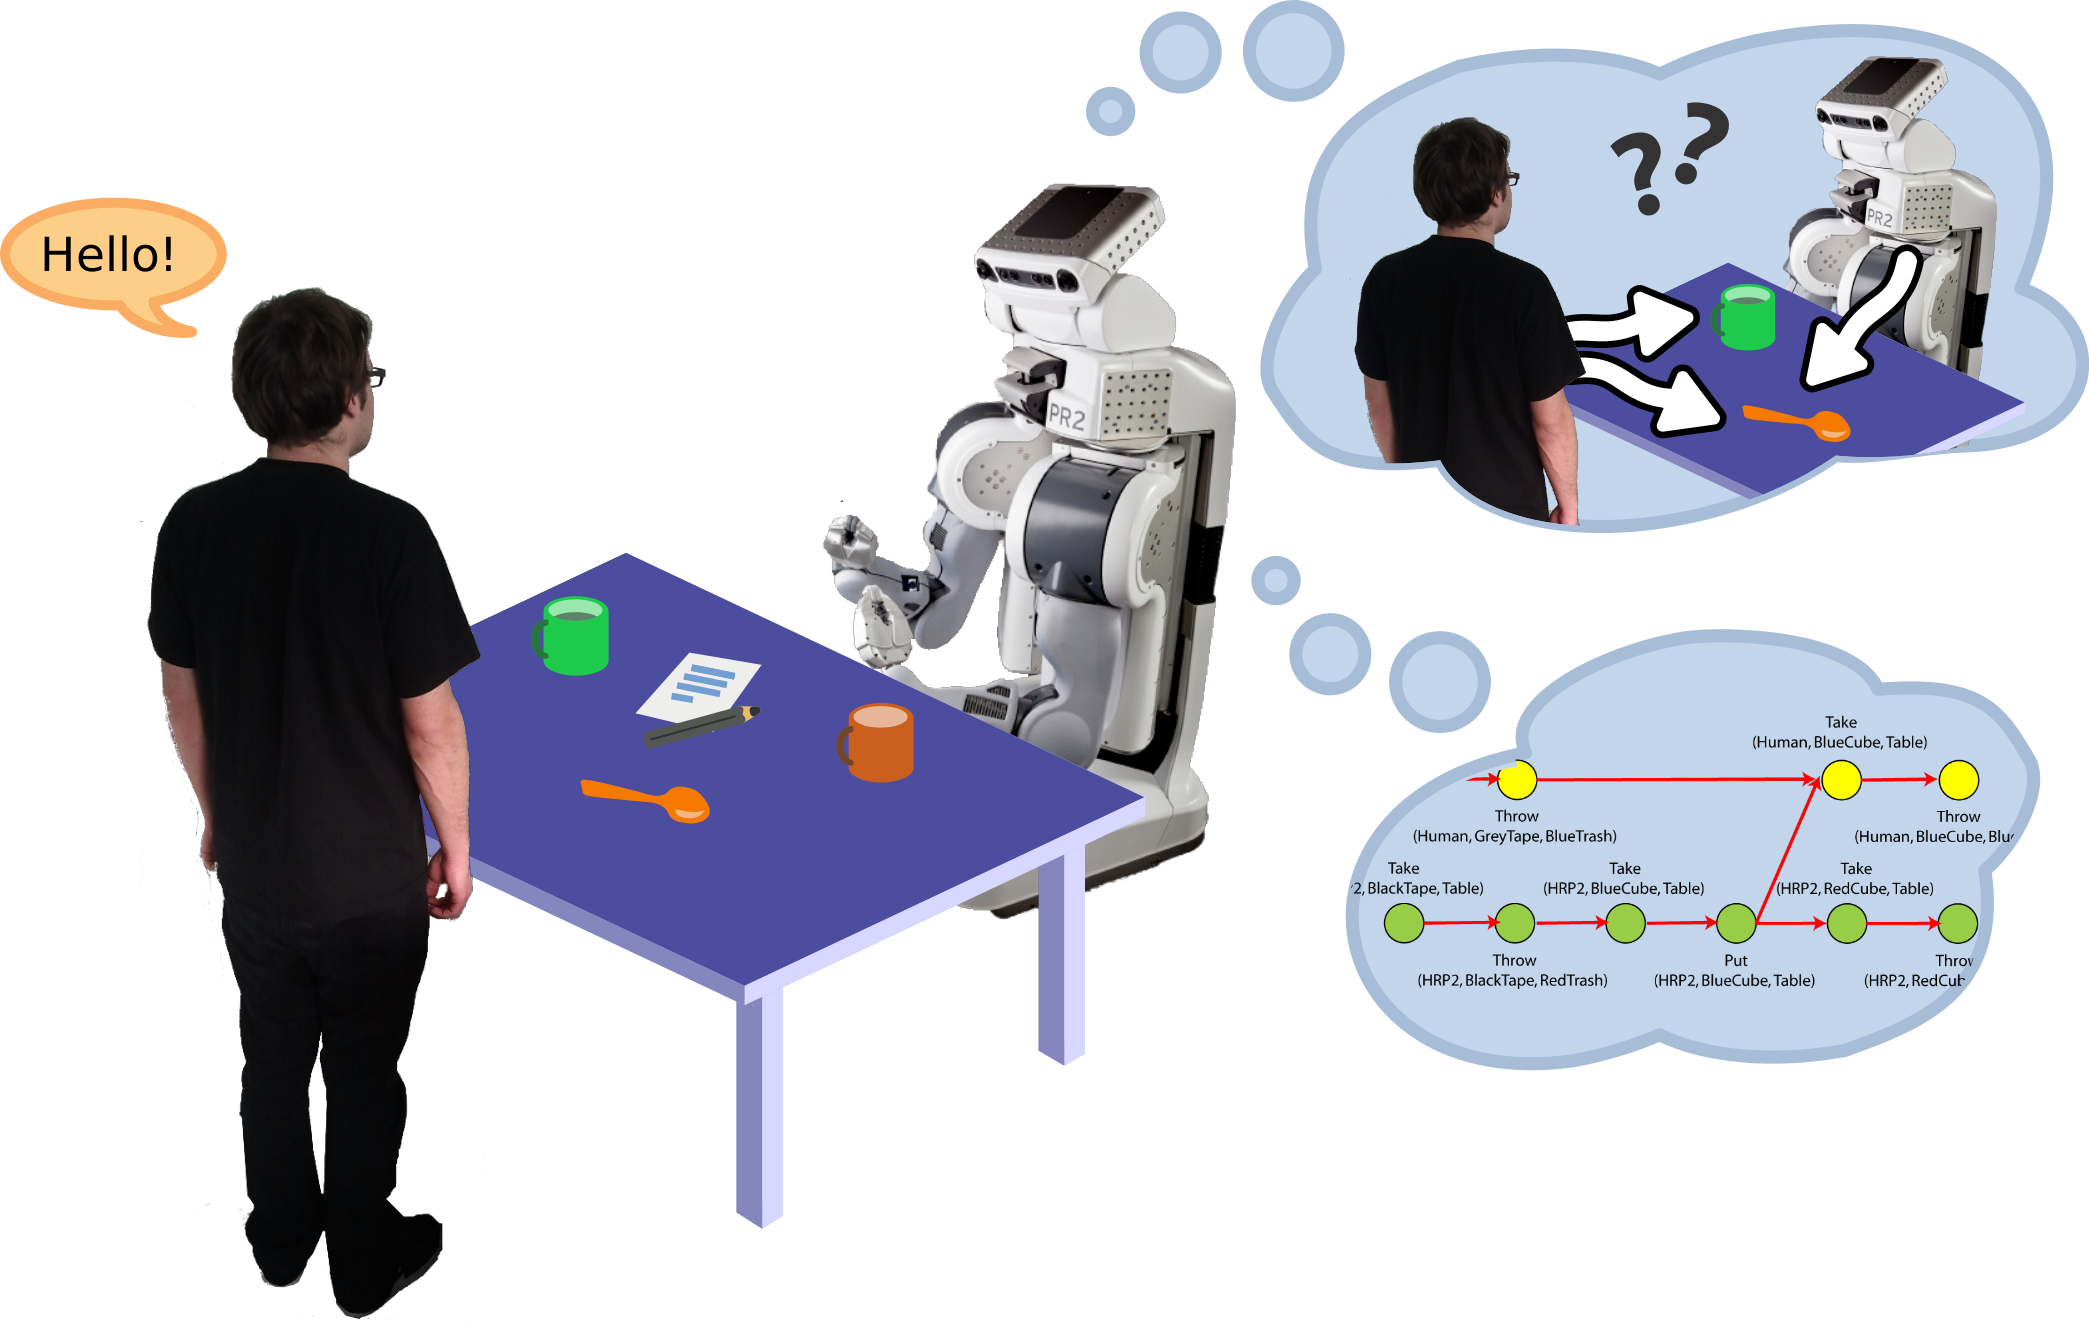
\includegraphics[width=0.6\textwidth]{grounding_robot.png}};
    \node[circle, draw] at (-3.5,2.5) {A};
    \node[circle, draw] at (5.5,2) {D};
    \node[circle, draw] at (5.2,-1) {C};
    \node[circle, draw] at (-1,2) {B};
\end{tikzpicture}

\caption{The robot reasons and acts in domestic interaction scenarios.  The
    sources of information are multi-modal dialogue {\it (A)}, and
    perspective-aware monitoring of the environment and human activity {\it
    (B)}. The robot must adapt on-line its behaviours by merging computed plans
    with reactive control. The robot explicitly reasons on the fact that it is
    (or not) observed by the human. Reasoning and planning take place at
    symbolic {\it (C)} as well as geometric level and take into account agents
    beliefs, perspectives and capabilities {\it (D)} as estimated by the robot.}

\label{fig:hri-dec}
\end{figure}

\emph{Communication}, \emph{Joint Actions}, \emph{Human-Aware Execution}: these
three challenges structure the whole field of human-robot interaction research,
and can be analysed in terms of the cognitive skills that they require.

A \emph{joint action}, for instance, builds from:

\begin {itemize}
    \item a joint \emph{goal}, which has been previously established and agreed
        upon (typically through dialogue),
    
    \item a physical environment, estimated through the robot's exteroceptive
        sensing capabilities, and complemented by inferences drawn from previous
        observations,
    
    \item a belief state that includes {\it a priori} common-sense knowledge and
        mental models of each of the interactors.

\end {itemize}

The robot controller then decides on an action to execute next and who has to
perform it, from the human, the robot or both in case of a joint action, and
eventually controls or monitors its execution. The operation continues until the
goal is achieved, is declared unachievable or is abandoned by the human.

\begin{inparaenum}
This translates into several decisional, planning, representation skills that
need to be available to the robot. It must be able \item to represent and
manipulate symbolic belief states, \item to acquire and maintain them up-to-date
with respect to state of the world and the task at hand, \item to build and
maintain, and iteratively refine shared (human-robot) plans, \item to
instantiate and execute the actions it has to perform, and conversely,
to monitor those achieved by its human partner.
\end{inparaenum}

Such abilities must be designed and implemented in generic ways and
provide several levels of parametrization such as they adapt to
various environments, different tasks and variable levels of engagement of the
robot, ranging from teammate behaviour to assistant or proactive helper.

\subsection{Article organization}

The remaining of the article discusses the robotic architecture we have built to
tackle the AI challenges of human-robot interaction, and how its relates to
other approaches. We propose to organise this discussion in four sections.

The next section presents the overall architecture and the knowledge model we
have developed for our robots. Section~\ref{sec:impl} gives some insights on
each of the main components of the architecture, and try to highlight their
significance for artificial intelligence. Section~\ref{sec:expe} presents two
experiments that illustrate in a concrete way what can be currently achieved
with our robots.  Section~\ref{sect|conclusion} finally summarises our main
contributions and relate them to other recent researches in the field.

\section{Deliberative Architecture and Knowledge Model}


\begin{figure*}[ht]
\centering

\resizebox{\textwidth}{!}{%

\tikzset{subpart/.style={draw, font=\scriptsize, fill opacity=0.5, text opacity=1, fill=black!50}}

\begin{tikzpicture}[
    >=latex,
    every edge/.style={draw, very thick},
    skill/.style={draw, rounded corners, align=center, inner sep=5pt, fill=black!20},
    label/.style={midway, align=center, font=\scriptsize, fill=white}]

  %%% ORO
    \node at (0,0)[skill, ultra thick, fill=LimeGreen!50] (oro) {{\sc Oro} -- Symbolic facts \\ and beliefs management};
  
  %%% HATP
  \node at (-6, 2)[skill, fill=PineGreen!50] (hatp) {HATP -- Human-aware \\ symbolic task planning};
  
  %%% DIALOGS
  \node at (-6, -2) [skill, fill=BrickRed!50] (dialogs) {{\sc Dialogs} \\ Dialogue processing};

  %%% SPARK
  \node at (4,-3)[skill, fill=Purple!50] (spark) {%
      \begin{tikzpicture}
          \node at (0,0) (geom) {{\sc Spark} -- Geometric \& Temporal Reasoning};
        \node [subpart, below=0.2 of geom.south west, anchor=north west] (world-update) {Sensors fusion};
        \node [subpart, right=0.2 of world-update] (geom-model) {Geometric model of the environment};
        \node [subpart, right=0.2 of geom-model] (fact-prod) {Symbolic facts production};
      \end{tikzpicture}
    };

  %%% MHP
    \node at (9,0)[skill, fill=BurntOrange!50] (mhp) {{\sc mhp} -- Human-aware \\ Motion and Manipulation \\ Planning};

  %%% SHARY
  \node at (4,4)[skill, fill=RoyalBlue!50] (shary) {%
      \begin{tikzpicture}
        \node at (0,0) (exec) {Execution Controller};
        \node [subpart, below=0.2 of exec.south west, anchor=north west] (plans) {Goal \& Plans \\ management};
        \node [subpart, right=0.2 of plans] (sit-asses) {Situation assessment \\ and context management};
        \node [subpart, right=0.2 of sit-asses] {Action instantiation, \\ execution and monitoring};
      \end{tikzpicture}
    };


  %%% LOWLEVEL
  \node [skill, below=of spark] (lowlevel) {%
      \begin{tikzpicture}
        \node at (0,0) (sensori) {Sensorimotor layer};
        \node [subpart, below=0.2 of sensori.south west, anchor=north west, align=left] (perception) {{\bf Perception} \\ 2D markers, RGB-D, motion capture};
        \node [subpart, align=right, right=0.2 of perception] {{\bf Actuation} \\ Head's pan-tilt unit, grippers, arms, wheels};
      \end{tikzpicture}
  };

  %%% Separation between deliberative layer and sensori-motor layer
  \draw[dotted, thick] (-8,-4.5) -- (12, -4.5);

  %%% Relations between components
  \path (shary.340) edge [<->, bend left] node[label] {motion plan \\ requests} (mhp);
  \path (shary.west) edge [<->, bend right] node[label] {shared \\ plans} (hatp);
  \path (hatp) edge [<->, bend right] node[label] {world model and \\ agents beliefs} (oro.170);
  \path (dialogs) edge [<->, bend left] node[label] {natural language \\ grounding} (oro.190);
  \path (spark.100) edge [->, bend right] node[label] {symbolic \\ facts} (oro);
  \path (shary) edge [<->, bend left] node[label] {events, \\ world model and \\ agents beliefs} (oro);
  \path (shary) edge [<->, bend left] node[label] {action monitoring \\ and management of \\ position hypotheses} (spark);
  \path (lowlevel) edge [->] (spark);
  \path (lowlevel.east) edge [<-, bend right=80, looseness=1.2] (shary.east);

\end{tikzpicture}
}

\caption{Overview of the architecture. The deliberative layer (on the top),
composed of six main modules, interacts with the low-level sensori-motor
layer (on the bottom). Knowledge is centrally managed in an active
\emph{semantic blackboard}, pictured above with a thick border. The links
between components depicted on the figure underline the central role of the
knowledge base: most of the datastreams are actually symbolic statements exchanged
through the semantic blackboard.}


    \label{fig|archi}
\end{figure*}

\subsection{Building a human-aware deliberative layer}

Connecting multiple independent software modules in one coherent robotic
architecture is not only a technical challenge, but also a design and
architectural challenge.

In particular, dealing with the rich semantics of natural interaction with
humans has been one of our major focus. To this end, we have been deploying
over the last years explicit knowledge representation and manipulation in the
deliberative layer of the robots as a {\it lingua franca} between our
components.

Figure~\ref{fig|archi} gives an overview of our architecture. An active
knowledge base ({\sc Oro}), conveniently thought as a \emph{semantic
blackboard}, connects most of the modules together: the \emph{geometric
reasoning} module (called {\sc Spark}) produces symbolic assertions (like
\stmt{BOOK1 isOn TABLE}) describing the state and dynamics of the robot's
environment. These logical statements are stored in the knowledge base, and
reused by the language processing module ({\sc Dialogs}), the symbolic task
planner (HATP) and the execution controller. The output of the language
processing module, or the activities started by the robot controller are
likewise stored as symbolic statements.

For instance, when processing a sentence like ``give me another book'', the {\sc
Dialogs} module sends at some point a request to the knowledge base that looks
like {\tt \footnotesize find(?book type Book, ?book differentFrom
BOOK1)}\footnote{We present a similar but complete example at
section~\ref{moving-london}.} and may write back assertions like \stmt{HUMAN
desires GIVE\_ACTION45, GIVE\_ACTION45 actsOn BOOK2} to {\sc Oro}. The HATP
planner then uses the knowledge base to initialise the planning domains with
similar requests ({\tt \footnotesize find(BOOK2 isAt ?location)}, etc.). The
execution controller typically monitor conditions (by subscribing to events
like: {\tt \footnotesize onNewMatch(HUMAN desires ?goal)}) and stores what the
robot is currently doing (\stmt{myself currentlyPerforms GIVE\_ACTION45}).

To some extend, this architecture moves away from classical layered approaches
found in robotics~\cite{Gat1998three, Volpe2001CLARAty, Goldberg2002}.
Interactions between components at the deliberative level are mostly
bidirectional and we do not introduce layers of abstraction amongst software
components\footnote{We do have lower-level modules to execute actions or manage
sensors, but all cognition-related modules live in the same global deliberative
layer.}. Dialogue processing, for instance, illustrates this structure. This
component does not purely act as an alternative sensing modality that would be
fed to a distinct deliberative component: on the contrary, it actively queries
the knowledge base to interpret and disambiguate natural language, and in that
regards, it is fully integrated to the deliberative process itself (we detail
natural language processing at section~\ref{sect|com}).

Our architecture however relates to \emph{Beliefs, Desires, Intentions} (BDI)
architectures. As put by Woolridge~\cite{Woolridge1999}, BDI architectures are
primarily focused on \emph{practical reasoning}, \ie the process of deciding,
step by step, which action to perform to reach a goal. The management of the
interaction between knowledge (the beliefs) and task and plan representation and
execution (the desires and the intentions) is central, and aims at selecting at
each step the best sub-goal. It becomes then an intention that the robot commits
to.

As for any cognitive system, this fundamental interaction between knowledge and
actions is central to our approach, and involves the dialogue component that
acquires \emph{desires} from the other agents, the planner and the execution
controller that may first decide to take or not into account an incoming desire
as a \emph{goal}, and then generates and manages \emph{intentions} from these
goals with the help of a symbolic task planner.

Other activities are however conducted in parallel, without being explicitly
triggered by \emph{desires} in the BDI sense, like situation assessment and
monitoring or other forms of dialogue (including performative dialogue that can
possibly change the internal state of the robot, but does not lead directly to
the creation of \emph{desires}, like assertion of new facts or question
answering).

\subsection{Knowledge Model}

In our architecture, knowledge manipulation relies on a central server (the {\sc
Oro} server~\cite{Lemaignan2010}, Figure~\ref{fig|spark-oro} top) which stores
knowledge as it is produced by each of the deliberative components (the
clients). It exposes a {\tt json}-based RPC API~\cite{lemaignan2012kbapi} to
query the knowledge base. The clients of the {\sc Oro} server are in charge of
managing themselves the knowledge (when to add, when to update, when to
retract knowledge): no meta-semantics is carried over that would let the server
manage these dynamics itself.\footnote{There is one exception: so-called
\emph{memory profiles} let the server discard facts after a specific period
of time. We present this experimental feature at section~\ref{memory}.} We
represent knowledge as RDF triples in the OWL sub-language. Each time
triples are added or removed from the knowledge base, a Description Logics
reasoner ({\sc Pellet}\footnote{\tt http://clarkparsia.com/pellet/})
classifies the whole ontology and inserts all possible inferred triples.

This architecture design (a central knowledge base that essentially appears as a
passive component to the rest of the system -- even though it actually actively
processes the knowledge pool in the background, for instance with the reasoner)
departs from other approaches like the CAST model~\cite{Hawes2007} where
knowledge is represented as a diffuse resource, or the CRAM/KnowRob
architecture~\cite{Beetz2010} where the knowledge base is an active hub that
pro-actively queries perceptual components to acquire knowledge. We believe that
our design leads to a good \emph{observability} (knowledge flows are explicit
and easy to capture since they are centralised) as well as high modularity
(modules communicate through a defined and unified API).

At run-time, the knowledge available to the robot at a given time comes from
three sources. {\it A priori} knowledge is stored in an ontology (the {\sc
OpenRobots} ontology, discussed below) and loaded at start-up. This static source covers the
\emph{common-sense} knowledge of the robot, and optionally some
scenario-specific knowledge (for instance, about objects that are to be
manipulated). The second part of the knowledge is acquired at run-time from
perception, interaction and planning. The next sections detail these processes.
Lastly, the third source of symbolic statements is the reasoner itself.

Contrary to other projects like KnowRob~\cite{Tenorth2009a} that relies on
the concept of \emph{computables} to lazily evaluate/acquire symbolic facts when
needed, we have an \emph{explicit} approach where we greedily compute and assert
symbolic statements (like spatial relations between objects, see
Section~\ref{sect|sit-ass}). This design choice trades scalability for explicit
reasoning: at any time, the full belief state is explicitly stated, and
provides the reasoner with the largest possible inference domain. This is of
special importance for an \emph{event-based} architecture like ours (see
Section~\ref{sect|ctrl}), where, by definition, we do not know beforehand what
we are ``looking for'', and we need instead greedily infer as much as possible
to build a belief state as comprehensive as possible.

\begin{figure}
    \centering

\resizebox{0.8\textwidth}{!}{%
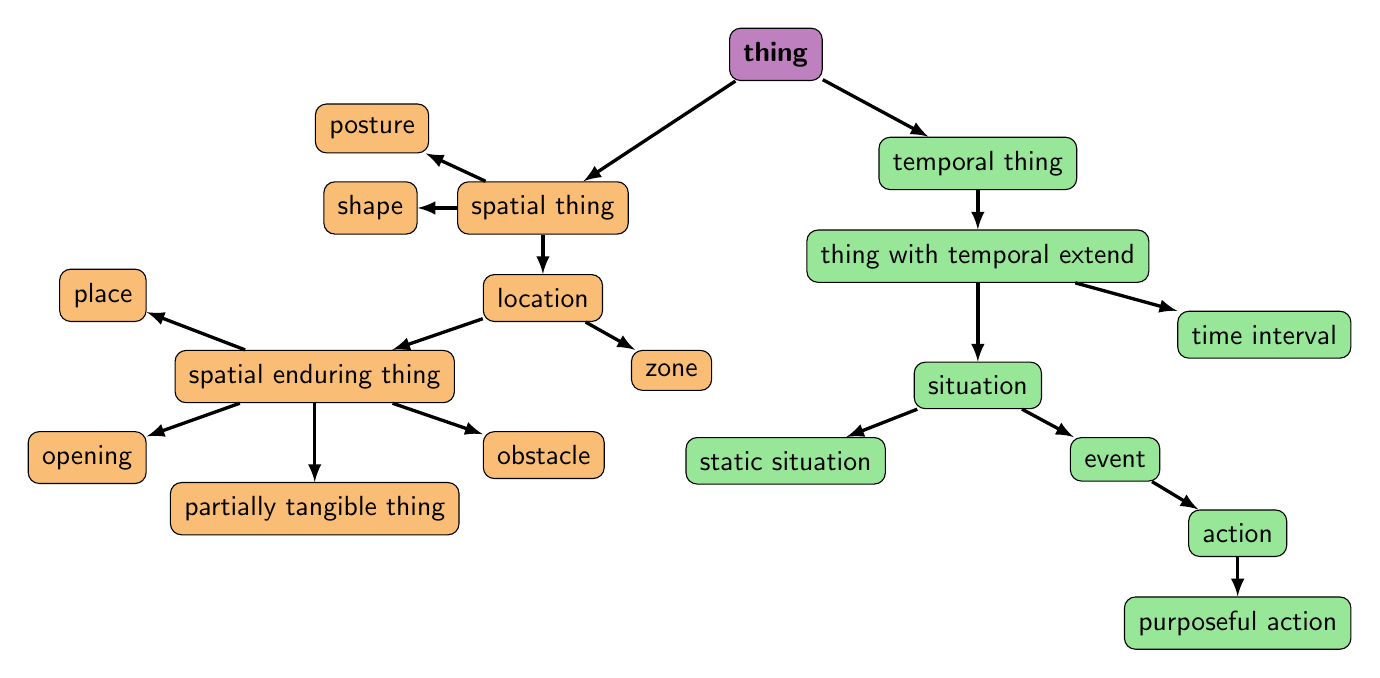
\begin{tikzpicture}[
    >=latex,
    every edge/.style={<-, draw, very thick},
    every node/.style={draw, font=\sf, node distance=0.5, rounded corners,
align=center, inner sep=5pt,fill=LimeGreen!50}]

    \node[fill=Purple!50] (thing) {\textbf{thing}};
    \node [fill=BurntOrange!50, node distance=1.8, below left=of thing](sthing) {spatial thing} edge (thing);
        \node [fill=BurntOrange!50, above left=of sthing] {posture} edge (sthing);
        \node [fill=BurntOrange!50, left=of sthing] {shape} edge (sthing);
        \node [fill=BurntOrange!50, below=of sthing] (location) {location} edge (sthing);
            \node [fill=BurntOrange!50, below right=of location] {zone} edge (location);
            \node [fill=BurntOrange!50, below left=of location] (set) {spatial enduring thing} edge (location);
                \node [fill=BurntOrange!50, below right=of set] {obstacle} edge (set);
                \node [fill=BurntOrange!50, below left=of set] {opening} edge (set);
                \node [fill=BurntOrange!50, below=1 of set] {partially tangible thing} edge (set);
                \node [fill=BurntOrange!50, above left=of set] {place} edge (set);

    \node [node distance=1, below right=of thing] (tthing) {temporal thing} edge (thing);
        \node [below=of tthing] (tte) {thing with temporal extend} edge (tthing);
            \node [below right=of tte] {time interval} edge (tte);
            \node [below=1 of tte] (sit) {situation} edge (tte);
                \node [below right=of sit] (evt) {event} edge (sit);
                    \node [below right=of evt] (act) {action} edge (evt);
                        \node [below=of act] {purposeful action} edge (act);
                \node [below left=of sit] {static situation} edge (sit);

\end{tikzpicture}
}

\caption{The upper part of the {\sc Oro} common-sense TBox. All these concepts
    belong to the {\sc OpenCyc} namespace.}
    
    \label{fig|upper_tbox}
\end{figure}

\paragraph{The OpenRobots Ontology} The {\sc Oro} common-sense ontology has been
designed from two requirements: covering our experimental needs and conforming
as much as possible to the {\sc OpenCyc} upper ontology.

This leads to a bidirectional design process: from \emph{bottom-up} regarding
the choices of concepts to model, \emph{top-down} regarding the upper part of
the taxonomy. This upper part of the ontology is pictured on
Figure~\ref{fig|upper_tbox}. All the classes visible in this figure belong to
the {\sc OpenCyc} namespace.

Aligning the upper part of the ontology on {\sc OpenCyc} (as done by other
knowledge representation systems, like {\sc KnowRob}~\cite{Tenorth2009a} or PEIS
K\&R~\cite{Daoutis2009}) has multiple advantages. First the design of this part
of the ontology is generally difficult: it pertains to abstract concepts whose
mutual relations comes to philosophical debates. The upper taxonomy of {\sc
OpenCyc} represents a relative consensus, at least within the semantic Web
community. Then, because it is a well established project with numerous links to
other on-line databases (like Wikipedia or WordNet), the reuse of important {\sc
OpenCyc} concepts ensures to a certain extend that the knowledge stored by the
robot can be shared or extended with well-defined semantics. A good example is
the concept of \emph{Object}: In everyday conversation, an object is a
relatively small physical thing, that can be typically manipulated. Normally, a
human is not considered as an object. In {\sc Cyc}, an object has a more precise
definition: it is something \emph{partially tangible}. That includes obviously
the humans, and actually many other entities that would not be commonly said to
be objects (the Earth for instance). Thus the importance of relying on
well-defined and standard semantics to exchange informations between artificial
systems.

Figure~\ref{fig|upper_tbox} also illustrates the fundamental disjunction
in the {\sc Oro} model between \emph{temporal} and \emph{spatial} entities (formally,
$(\text{TemporalThing} \sqcap \text{SpatialThing})^{\mathcal{I}} = \emptyset$, with
$\mathcal{I}$ the \emph{interpretation} of our model).

The class \concept{PurposefulAction} is the superset of all the actions that are
purposefully performed by the robot (or another agent). Actual actions (\ie
subclasses of \concept{PurposefulAction} like \concept{Give} or
\concept{LookAt}) are not initially asserted in the common-sense ontology. They
are instead added at run-time by the execution controller (in link with the
symbolic task planner) and the natural language processor based on what the
robot is actually able to perform and/or to interpret in the current context
(\ie the current robot configuration and the actions required by the scenario).
The set of actions that the robot can interpret typically corresponds to the
planing domain in use: the robot can only process the \concept{GoTo} action if
the corresponding task description with its pre- and post-conditions is
available to the symbolic task planner.

The tree in Figure~\ref{fig|upper_tbox}\footnote{This subset of the ontology is
indeed a tree. This has however not to be the case in general, and, as a matter
of fact, the TBox of the whole {\sc Oro} common-sense ontology does not form a tree}
is not equally developed in each directions at lower levels. The descendants of
\concept{PartiallyTangibleThing} (\ie what we commonly call \emph{objects}), for
instance, are pictured in Figure~\ref{fig|tangible_things_tbox}. This excerpt
from the ontology makes the bottom-up design process clear: only few types of
\emph{partially tangible} things appear, and those are only subclasses relevant
to the context of service robotics in an human-like environment. For performance
reasons as well as clarity, we do not attempt to pro-actively extend the
conceptual coverage of the field. We instead opportunistically extend the
common-sense knowledge when required by experiments.


\begin{figure}
    \centering

\resizebox{0.5\textwidth}{!}{%
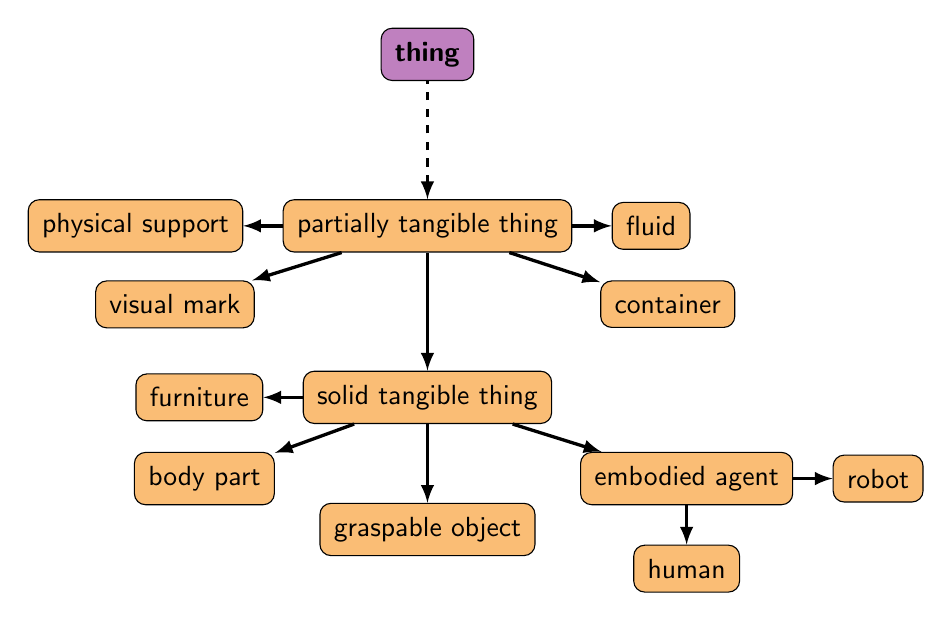
\begin{tikzpicture}[
    >=latex,
    every edge/.style={<-, draw, very thick},
    every node/.style={draw, font=\sf, node distance=0.5, rounded corners,
align=center, inner sep=5pt,fill=BurntOrange!50}]

    \node[fill=Purple!50] (thing) {\textbf{thing}};
    \node [below=1.5 of thing] (ptt) {partially tangible thing} edge[dashed] (thing);
        \node [left=of ptt] {physical support} edge (ptt);
        \node [below left=of ptt] {visual mark} edge (ptt);
        \node [below right=of ptt] {container} edge (ptt);
        \node [right=of ptt] {fluid} edge (ptt);
        \node [below=1.5 of ptt] (stt) {solid tangible thing} edge (ptt);
            \node [below=1 of stt] {graspable object} edge (stt);
            \node [below left=of stt] {body part} edge (stt);
            \node [left=of stt] {furniture} edge (stt);
            \node [below right=of stt] (ea) {embodied agent} edge (stt);
                \node [below=of ea] {human} edge (ea);
                \node [right=of ea] {robot} edge (ea);

\end{tikzpicture}
}
    \caption{TBox of the specialisations of \concept{PartiallyTangibleThing}.}
    \label{fig|tangible_things_tbox}
\end{figure}

Lastly, the {\sc Oro} common-sense ontology contains several rules and class
expressions that encode non-trivial inferences. The definition of
\concept{Bottle} as found in the {\sc Oro} ontology is a typical example:

\concept{Bottle} $\equiv$ \concept{Container} {\bf and} \concept{Tableware}
{\bf that} (\concept{hasShape} {\bf value} \concept{cylinderShape} {\bf and}
\concept{hasCharacteristicDimension} {\bf only} \concept{\em int[>= 0.1, <=
0.3]})

If a human informs the robot that a given object is indeed a bottle, the robot
can then derive a few more informations on this object. And, conversely, if the
human affirms that a car is a bottle, the robot may question this assertion
because of the inconsistent size (the {\sc Dialogs} module relies on such
logical consistency checks when processing natural language inputs, both to
ensure that the verbal input has been correctly acquired and to verify that what
the human says does actually make sense).

We will come back and discuss in section~\ref{krs-discussion} the strengths and
weaknesses of this knowledge framework.

\subsection{Symbol Grounding}

\emph{Grounding} (also called \emph{anchoring} when specifically referring to
the building of links between \emph{percepts} and \emph{physical
objects}~\cite{Coradeschi2003}) is the task consisting in building and
maintaining a bi-directional link between sub-symbolic representations (sensors
data, low-level actuation) and symbolic representations that can be manipulated
and reasoned about~\cite{Harnad1990}. This represents an important cognitive
skill, in particular in the human-robot interaction context: in that case, the
link that the robot has to established between its percepts and its symbol must
\emph{model} to a large extend the human representations in order to effectively
support communication.

\emph{Symbol grounding} relates the knowledge model to the perception and
actuation capabilities of the robot, and our architecture adopts here a
bidirectional approach.  The different components that we have described so far
provide a \textit{bottom-up} grounding process: geometric reasoning and dialogue
processing modules constantly build and push new symbolic contents about the
world to the knowledge base where it becomes accessible to decisional layers. In
parallel, the knowledge base relies on reasoning in a \textit{top-down} way to
produce new facts, \ie new beliefs that may lead to actual decision making and
physical actions.


%%%%%%%%%%%%%%%%%%%%%%%%%%%%%%%%%%%%%%%%%%%%%%%%%%%%%%%%%%%%%%%%%%%%%%%%%%%%%%%%
\section{Cognitive Skills}
\label{sec:impl}

While the previous section provided an overview of our cognitive architecture
as well as its associated knowledge model, this section discusses each of its main
``building blocks''. Each of these components may have connections to several
others, and we invite the reader to refer to Figure~\ref{fig|archi} as a guide
if needed.

\begin{inparaenum} In our context, we call \emph{cognitive skills} the
deliberative behaviours that are \item \emph{stateful} both in terms of
\emph{time} (keeping track of previous states is required for the component
to perform adequately) and \emph{modalities} (for instance, \emph{situated}
dialogue requires interleaving different communication modalities), \item
manipulate \emph{explicit semantics}, typically by the mean of symbolic
reasoning, \item operate at the \emph{human-level}, \ie are legible to the
humans, typically by acting at similar levels of abstraction.\end{inparaenum}

We start by discussing first the main \emph{internal} cognitive capabilities,
implemented in the knowledge base itself, and then discuss successively the
situation assessment module {\sc Spark}, the dialogue processor {\sc Dialogs},
the symbolic task planner HATP, and finally the main features of our execution
controllers.

\subsection{Internal Cognitive Skills}
\label{sect|intern}

We call \emph{internal} those cognitive capabilities that are tightly bound to
the knowledge model, and hence implemented directly within the {\sc Oro} server.
We present here three of them: \emph{reasoning}, \emph{theory of mind} modelling
and our (naive) approach to \emph{memory management}.

\subsubsection{Reasoning}
\label{reasoning}

As mentioned in the previous section, we use the Pellet open-source reasoner to
reason on the knowledge base. This enables several standard inference services:
\emph{consistency checking}, \emph{concept satisfiability},
\emph{classification} and \emph{realisation} (computation of the most specific
classes that an individual belongs to). In case of logical inconsistency, the
reasoner can also provide \emph{explanations} that are important for debugging.

Besides those, {\sc Oro} server implements several algorithms to identify
similarities and differences between concepts (classes or
instances)~\cite{Ros2010b}: the \emph{Common Ancestors} algorithm, useful to
determine the most specific class(es) that include a given set of individuals;
the \emph{First Different Ancestors} algorithm that returns what can be
intuitively understood as the most generic types that \emph{differentiate} two
concepts; and \emph{clarification} and \emph{discrimination} algorithms that
play a key role in the process of \emph{interactive grounding} of the semantics
of concepts (we discuss this process at section~\ref{sect|com}). Clarification
and discrimination algorithms are based on what we call \emph{descriptors}, \ie
properties of individuals, either statically asserted in the common-sense
ontology, acquired by the robot through perception or proactive questioning of
the human partner, or derived from other reasoning algorithms like the
\emph{Common Ancestors} and \emph{Different Ancestors}. The
\emph{discrimination} algorithm consists then in looking for discriminants, \ie
descriptors that allow a maximum discrimination among a set of individuals.

\subsubsection{Theory of Mind}
\label{sect|tom}

Theory of Mind (originally defined in~\cite{Premack1978}) is the cognitive
ability that allows a subject to represent the mental state of another
agent, possibly including knowledge that contradicts the subject's own model: for
example, a book can be at the same time \emph{visible} for myself, and \emph{not
visible} for you. Children develop this skill, which is essential to understand others' perspectives during
interactions, around the age of three. 

From a robotics point of view, it supposes the ability to build, store and
retrieve separate models of the beliefs of the agents the robot interacts with.
Our knowledge base implements such a mechanism: when the robots recognises that
a new agent has been created in the knowledge base, it initialises a new,
independent, ontology for this agent. All the ontologies that are created share
the same common-sense knowledge, but rely on each agent's perspective for the
actual instantiation: the robot (geometrically) computes that the book is in its
own field of view, but not in the human one. The robot knowledge contains the
fact \stmt{book isVisible true} while the human model contains \stmt{book
isVisible false} (this computation, called \emph{perspective taking}, is
discussed in the next section).

One classical application of this cognitive skill is the so-called
\emph{False-Belief} experiment (also known as the \emph{Sally and Ann}
experiment)~\cite{Leslie2000}: a child is asked to watch a scene where two
people, A and B, manipulate objects. Then A leaves and B hides away one
object. When A comes back, we ask the child ``where do you think A will
look for the object?''. Before acquiring a theory of mind, children are not
able to separate their own (true) model of the world (where they know that
the object was hidden) from the model of A, which contains \emph{false
beliefs} on the world (A still thinks the object is at its original
position since he did not see B hiding it). Using separate knowledge models
in the knowledge base, we have been able to replicate this experience with
our robots~\cite{warnier2012when}.

\subsubsection{Working memory}
\label{memory}

Memory has been studied at length in the cognitive psychology and
neuropsychology communities: very briefly, the idea of \emph{short-term} and
\emph{long-term} memory is due to Atkinson and Shiffrin~\cite{Atkinson1968} ,
Anderson~\cite{Anderson1976} splits memory into \emph{declarative} (explicit)
and \emph{procedural} (implicit) memories, Tulving~\cite{Tulving1985} organises
the concepts of \emph{procedural}, \emph{semantic} and \emph{episodic} memories
into a hierarchy. Short-term memory is eventually refined with the concept of
\emph{working memory} by Baddeley~\cite{Baddeley2010}

It is worth emphasising that if memory is commonly associated to the process of
forgetting facts after a variable amount of \emph{time}, it actually covers
more mechanisms that are relevant to robotics, like selective remembering
triggered by a specific context or reinforcement learning.

The {\sc Oro} server features a mechanism to mimic only minimalistic forms of memory
families.  When new statements are inserted in the knowledge base, a
\emph{memory profile} is optionally attached to them.  Three such profiles are
predefined: {\tt short term}, {\tt episodic} and {\tt long term}. They are
currently attached to different lifetime for the statements (respectively 10
seconds, 5 minutes and no time limit). After this duration, the statements are
automatically removed from the knowledge base.

This approach is limited. In particular, \emph{episodic} memory should primarily
refer to the semantics of the statements (that is expected to be related to an
event) and not to a specific life duration.

We rely however on this mechanism in certain cases: for instance, some modules
like the natural language processor use the {\tt short term} memory profile to
mark for a few seconds important concepts that are currently manipulated by the
robot as \emph{active concepts}: If a human asks the robot ``Give
me all red objects'', the human, the \concept{Give} action, and each red
objects that are found are successively marked as \emph{active concepts} by
inserting statements such as \stmt{human type ActiveConcept} in the short-term
memory (which can be considered, in this case, to be a working memory). We use
this feature to trace certain knowledge-related processes.

In the larger field of cognitive architectures, the {\sc Soar}
architecture~\cite{Lehman2006} is one of those that tries to reproduce a
human-like memory organisation. The GLAIR cognitive
architecture~\cite{Shapiro2009} also has a concept of long term/short term and
episodic/semantic memories.


\subsection{Acquiring and Anchoring Knowledge in the Physical World}
\label{sect|sit-ass}

\begin{figure}
\centering
\resizebox{0.8\textwidth}{!}{%
\begin{tikzpicture}[
        >=latex,
        box/.style={draw,rectangle, dotted, minimum width=#1, minimum height=3.8cm},
        box/.default={4.5cm},
        every edge/.style={draw, ultra thick},
        every node/.style={align=center}]

    %\draw[step=1cm, draw=black!20] (-10,-5) grid (10,5);

    \node[draw=none] at (0,-1) {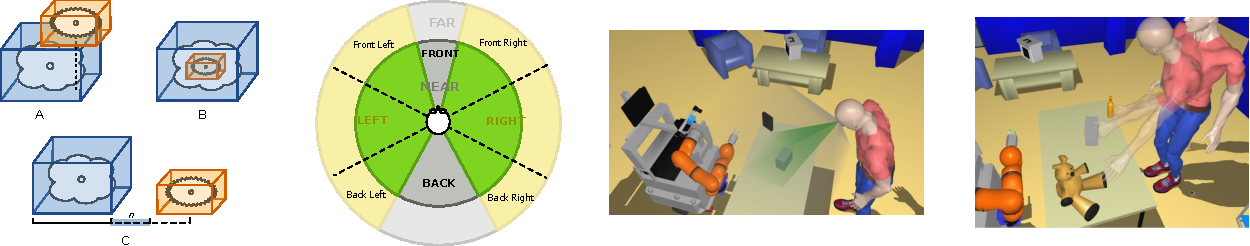
\includegraphics[width=0.8\columnwidth]{spark-oro-notext.pdf}};

    \node[box=16cm, minimum height=5.7cm, solid, thick, rounded corners] at (0,1.8) (oro) {};
    \node at (0,4.2) {\sc \Large oro-server};

    \node[anchor=south] at (-4.6,2.4) {Description Logics \\ (Open World assumption)};
    \node[box=3.7cm] at (-4.6,1.9) (owl) {};
    \node[anchor=south] at (-1,2.4) {Multiple simultaneous \\ symbolic models};
    \node[box=3.3cm] at (-1,1.9) (multi) {};
    \node[anchor=south] at (2.1,2.4) {Bio-inspired \\ memory};
    \node[box=2.7cm] at (2.1,1.9) (mem) {};
    \node[anchor=south] at (5,2.4) {Discrimination \& \\ categorization};
    \node[box=3cm] at (5,1.9) (disc) {};

    \node at (-3,-0.6) {{\it OWL store:} OpenJena};
    \node at (3,-0.6) {{\it Reasoner:} Pellet};

    %%%%%%%%%%%%%%%%%%%%%%%%%%%%%%%%%%%%%%%%%%%%%%%%%%%%%%%%%%%%%%%%%%%%%%%%%%%%%%%%%%%

    \node[box=16cm, minimum height=3.5cm, dotted, thick, rounded corners] at (0,-3.75) (spark) {};
    \path (spark.north) edge[->] node[align=left,anchor=west] {Symbolic\\facts} (oro.south);

    \node[anchor=north] at (-5.5,-4.5) {a) Agent-independent\\locations};
    \node[anchor=north] at (-1.8,-4.5) {b) Agent-dependent\\placements};
    \node[anchor=north] at (1.5,-4.5) {c) Visibility};
    \node[anchor=north] at (5.3,-4.5) {d) Reachability};

\end{tikzpicture}
}
    \caption{Functional overview of knowledge base ({\sc Oro} server, top part)
    and the geometric situation assessment module (\emph{{\sc Spark}}, bottom
    part). {\sc Spark} computes symbolic relationships between objects and
    agents, and feeds them to the knowledge base.}

        \label{fig|spark-oro}
\end{figure}

Anchoring perceptions in a symbolic model requires perception abilities and
their symbolic interpretation. We call \emph{physical situation assessment} the
cognitive skill that a robot exhibits when it assesses the nature and content of its
surroundings and efficiently monitors its evolution.

Numerous approaches exist, like amodal \emph{proxies}~\cite{Jacobsson2008},
grounded amodal representations~\cite{Mavridis2006}, semantic maps
(\cite{Nuechter2008, Galindo2008,Blodow2011}) or affordance-based planning and
object classification~\cite{Lorken2008, Varadarajan2011}.

%Spatial reasoning~\cite{O'Keefe1999} is a field in its own right, and has been
%used for natural language processing for applications such as direction
%recognition ~\cite{Kollar2010,Matuszek2010} or language
%grounding~\cite{Tellex2010}.~\cite{Skubic2004} present a spatial reasoner
%integrated in a robot which computes symbolic positions of objects.


We rely on a dedicated geometric and temporal reasoning module called {\sc
Spark} (\emph{SPAtial Reasoning \& Knowledge}~\cite{Sisbot2011}). It is a
situation assessment reasoner that generates symbolic knowledge from the
geometry of the environment with respect to relations between objects,
robots and humans (Figures~\ref{fig|spark-oro}
and~\ref{fig:sparkSubfigures}), also taking into account the different
perspective that each agent has on the environment.

{\sc Spark} is an \emph{amodal}~\cite{Mavridis2006} geometric model of the
environment that serves both as basis for the fusion of the perception
modalities and as bridge with the symbolic layer. This geometric model is
continuously updated at run-time by the robot based on its sensors (in our
experiments, objects are identified and localised through 2D fiducial markers, while
humans are tracked with Kinect-like devices, optionally assisted by motion
capture to accurately track the head motion, which is required to compute what
the human is looking at).

%Our approach, implemented in the {\sc Spark} module, is a grounded amodal
%representation of the robot environment, where different sensing modalities
%(vision-based fiducial markers tracking, RGBD human tracking, motion capture)
%are merged and where amodal spatial reasoning takes place (for instance,
%explanation generation for unexpected perceptions like a disappearing object).


From an artificial intelligence perspective, {\sc Spark} takes care of merging
sensing modalities, it computes and grounds perceptions into symbolic
knowledge (situation assessment), it is responsible for temporal interpretation of
situations and performs spatial perspective-taking.

{\sc Spark} is designed to run and continuously update the knowledge base (in our
experiments, it runs at about 10Hz). At each steps, it re-computes spatial
relationships and affordances for the whole scene, and send the delta (new
relations and relations that do not hold anymore) to the knowledge base. This
approach may raise scalability concerns (we did not however hit such issues in
our constrained scenarios), but greatly simplifies the management of the
\emph{dynamics} of the knowledge (\emph{When do I discard outdated knowledge?
When do I update it?}). Since it is equivalent to a reset of the reasoner
domain, it also hides issues linked to non-monotonic reasoning
(see~\cite{McCarthy2007} for a discussion on that question).


\begin{figure*}[ht!]
   \begin{center}
%
       \subfigure[Physical setting]{%
%           \label{fig:wuweiPhoto}
           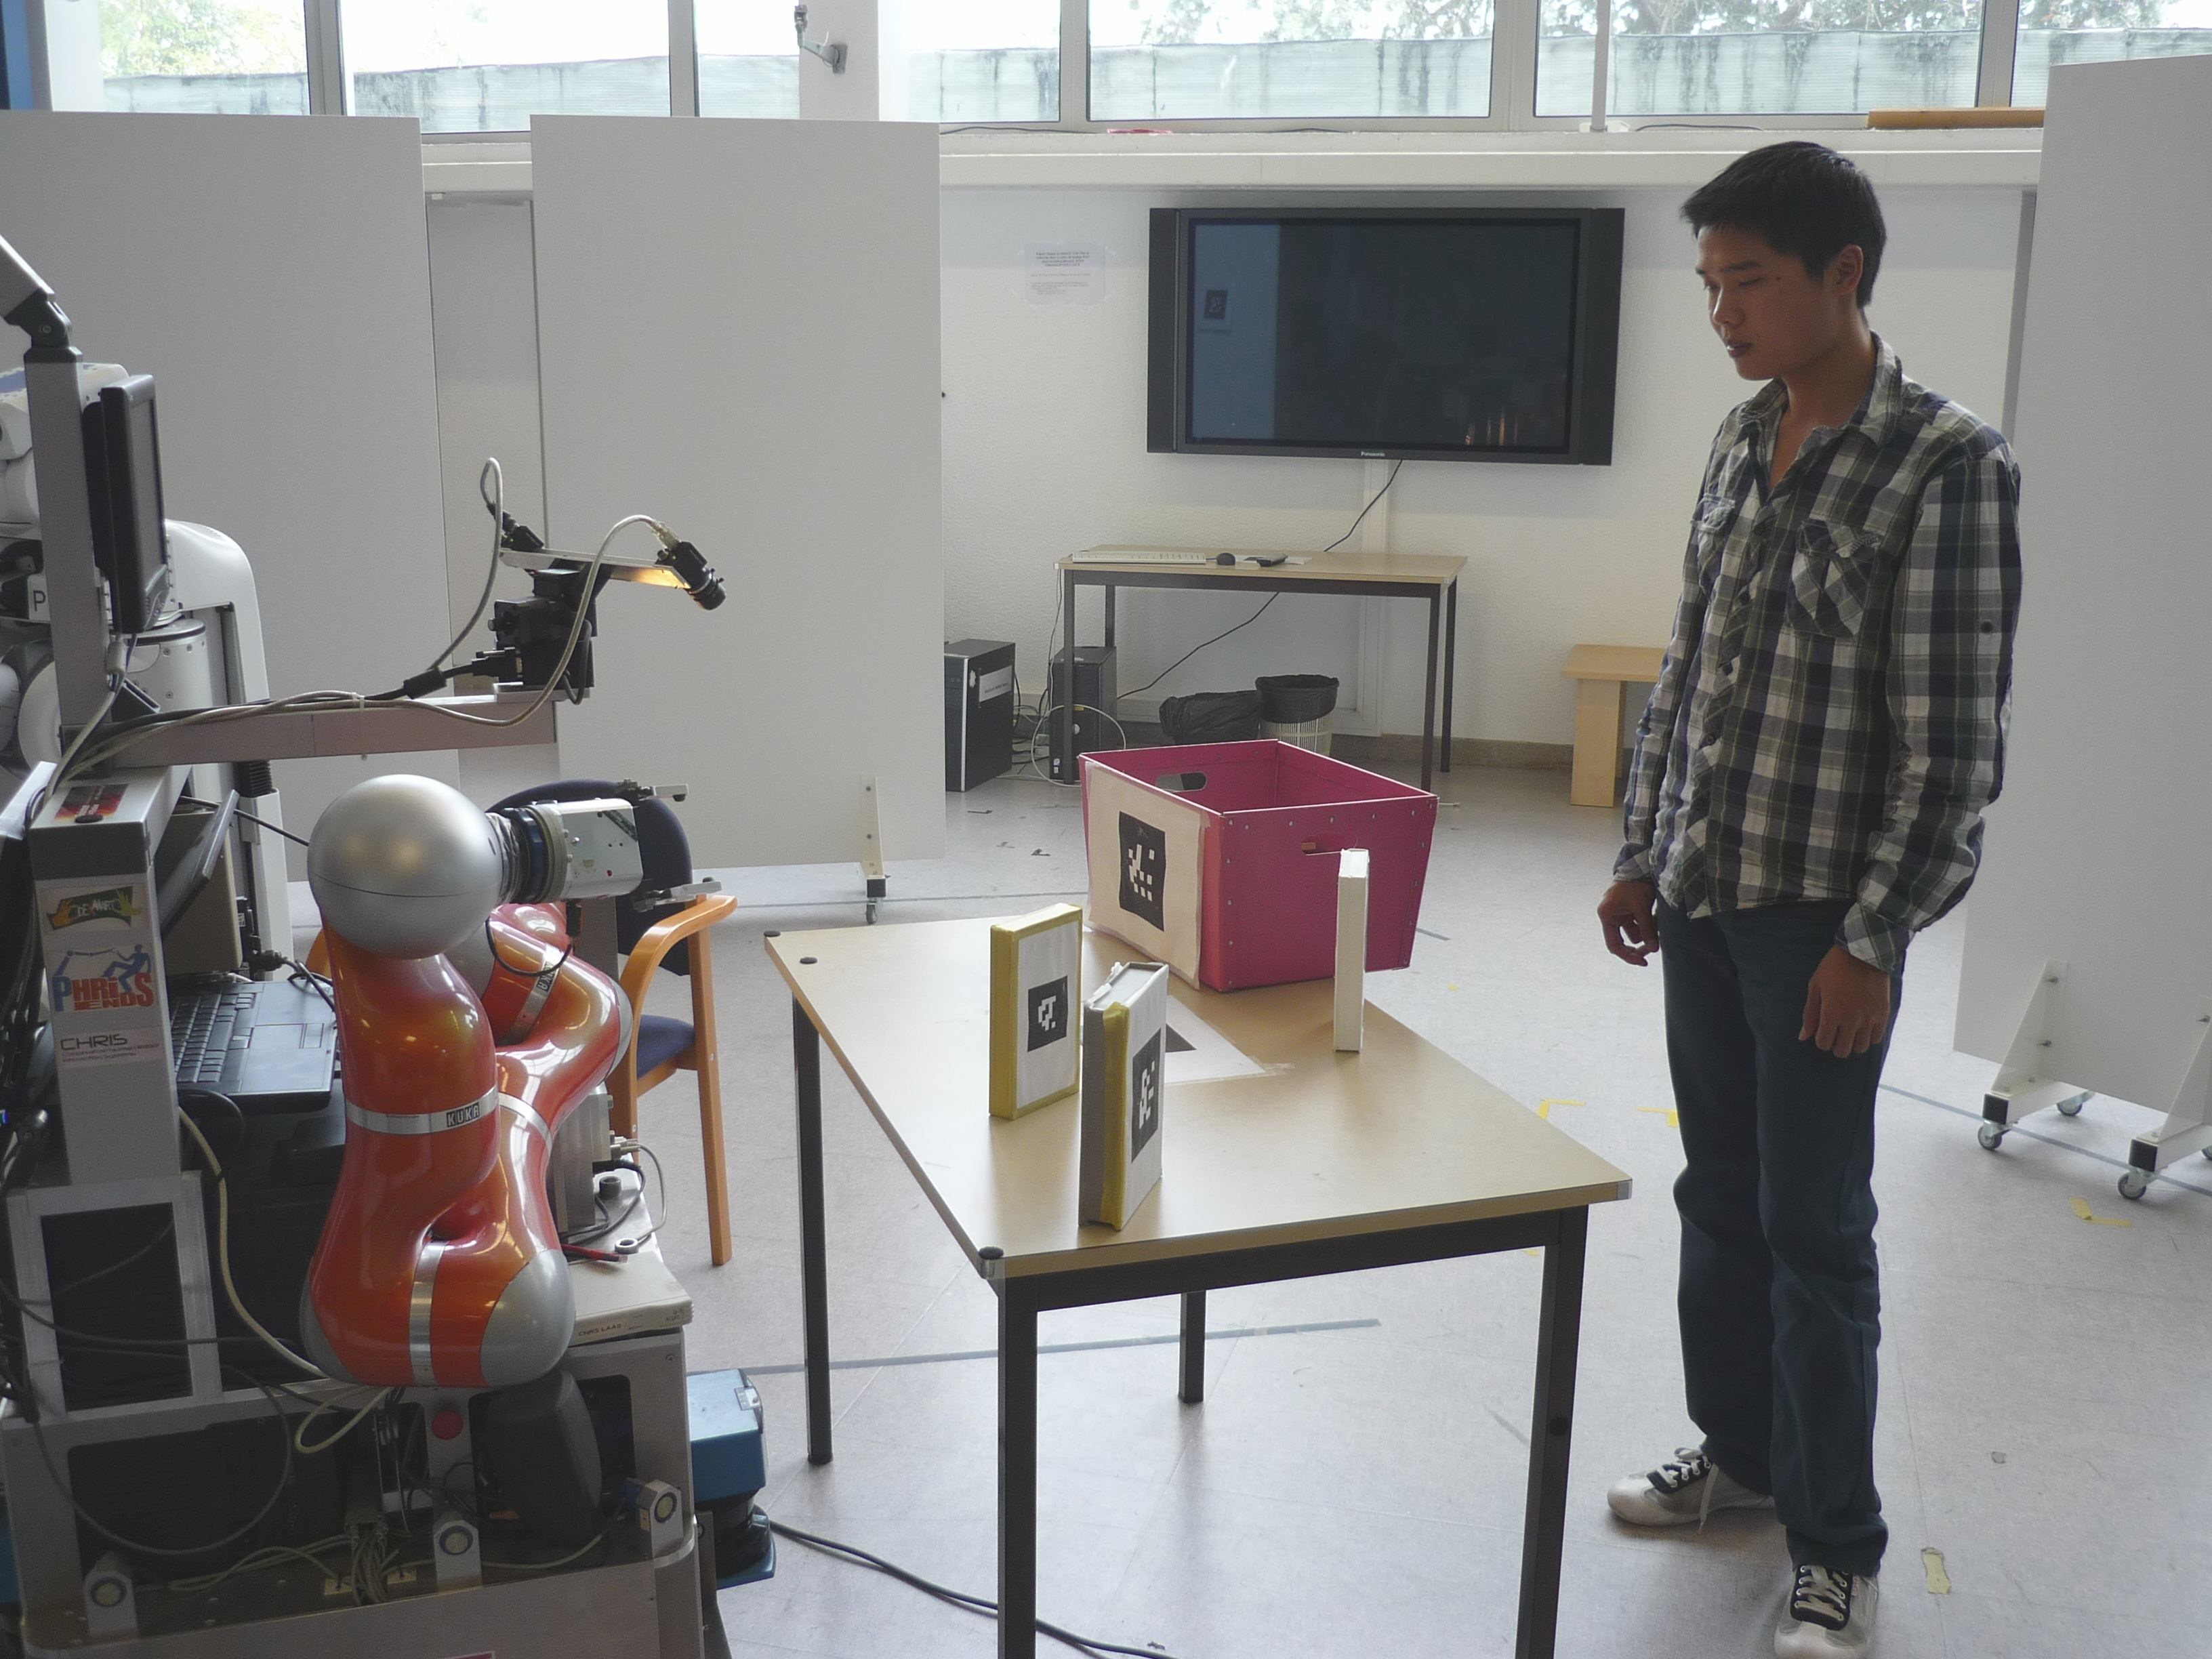
\includegraphics[width=0.5\textwidth]{etat2-P1010769_brightened-v2.jpg}
       }%
       \subfigure[Corresponding 3D model view]{%
%          \label{fig:sparkScreenshot}
          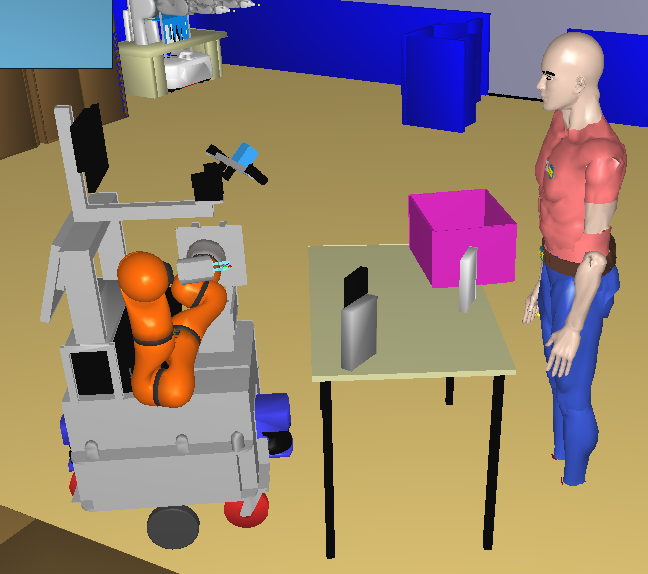
\includegraphics[width=0.43\textwidth]{etat2_photo.png}
       }\\ %  ------- End of the first row ----------------------%
%
   \end{center}

   \caption{Toy scenario involving videotapes that have to be manipulated, with
       other objects used as supports and containers.  After identification and
       localisation of the set of objects and acquisition of the position and
       posture of the human partner, the robot is able to compute that two tapes
       only are reachable by itself: the black and grey (in the 3D model) tapes.
       The third tape and the pink box are only reachable by the human. This
       situation leads to the symbolic model presented in
       Table~\ref{table|beliefsfig7}.  }%
        
 \label{fig:sparkSubfigures}

\end{figure*}

\begin{table}
\begin{center}
    \subfigure{
\begin{tabular}{l}
\hline
Robot's beliefs about itself (\emph{robot's model})\\
\hline
  \hspace{0.7cm}\stmt{PINK\_BOX isReachable false}\\
  \hspace{0.7cm}\stmt{WHITE\_TAPE isReachable {\bf false}}\\
  \hspace{0.7cm}\stmt{BLACK\_TAPE isReachable {\bf true}}\\
  \hspace{0.7cm}\stmt{GREY\_TAPE isReachable {\bf true}}\\
  \hspace{0.7cm}\stmt{WHITE\_TAPE isVisible true}\\
  \hspace{0.7cm}\stmt{BLACK\_TAPE isVisible true}\\
  \hspace{0.7cm}\stmt{GREY\_TAPE isVisible true}\\
  \hspace{0.7cm}\stmt{WHITE\_TAPE isOn TABLE}\\
  \hspace{0.7cm}\stmt{BLACK\_TAPE isOn TABLE}\\
  \hspace{0.7cm}\stmt{GREY\_TAPE isOn TABLE}\\
\hline
\end{tabular}
}\hspace{1em}%
\subfigure{
\begin{tabular}{l}
\hline
Robot's beliefs about the human (\emph{human's model})\\
\hline
  \hspace{0.7cm}\stmt{PINK\_BOX isReachable false}\\
  \hspace{0.7cm}\stmt{WHITE\_TAPE isReachable {\bf true}}\\
      \hspace{0.7cm}\stmt{BLACK\_TAPE isReachable {\bf false}}\\
      \hspace{0.7cm}\stmt{GREY\_TAPE isReachable {\bf false}}\\
  \hspace{0.7cm}\stmt{WHITE\_TAPE isVisible true}\\
  \hspace{0.7cm}\stmt{BLACK\_TAPE isVisible true}\\
  \hspace{0.7cm}\stmt{GREY\_TAPE isVisible true}\\
  \hspace{0.7cm}\stmt{WHITE\_TAPE isOn TABLE}\\
  \hspace{0.7cm}\stmt{BLACK\_TAPE isOn TABLE}\\
  \hspace{0.7cm}\stmt{GREY\_TAPE isOn TABLE}\\ 
 \hline
\end{tabular}
}
\end{center}
\caption{Symbolic facts computed from the situation depicted in
Figure~\ref{fig:sparkSubfigures}. Note how reachability differs for the two
agents.}

\label{table|beliefsfig7}
\end{table}

\subsubsection{Building an Agent-aware Symbolic Model of the Environment}
\label{sect|situ}

\paragraph{On Perspective Taking} Visual perspective taking refers to the
ability for visually perceiving the environment from other's point of view.
This ability allows us to identify the objects in situations where the visual
perception of one person differs from the other one. In developmental
psychology, one typical example consists of two similar objects in a room (\eg.
two balls) where both are visible for the child, but only one is visible for
the adult. Thus, when the adult asks the child to hand over ``the ball'', the
child is able to correctly identify which ball the adult is referring to (\ie
the one visible from the adult point of view), without asking~\cite{Moll2006}.

Besides, in order to compute a visual perspective, the actual visibility alone
is not enough. We include not only what the other person sees in a given
moment, but also what he \emph{can} see with a minimal effort (moving the eyes
or the head). To model the potential visibility of an object we compute a
visibility ratio while turning the head of the agent model towards the object.

Spatial perspective taking refers to the qualitative spatial location of
objects (or agents) with respect to a frame (\eg \emph{the keys on my left}).
Based on this frame of reference, the description of an object
varies~\cite{Marin2008}. Humans mix perspectives frequently during interaction.
This is more effective than maintaining a consistent one, either because the
(cognitive) cost of switching is lower than remaining with the same
perspective, or if the cost is about the same, because the spatial situation
may be more easily described from one perspective rather than
another~\cite{Tversky1999}. Ambiguities arise when one speaker refers to an
object within a reference system (or changes the reference system, \ie switches
perspective) without informing his/her partner about it~\cite{Breazeal2006,
Ros2010}. For example, the speaker could ask for the ``keys on the left''.
Since no reference system has been given, the listener would not know where
exactly to look.  However, asking for ``the keys on your left'' gives enough
information to the listener to understand where the speaker is referring to. On
the contrary, when using an exact, unambiguous term of reference to describe a
location (\eg. ``go north'') no ambiguity arises.

In {\sc Spark}, we use two types of the frames of reference: \emph{egocentric}
(from the robot perspective) and \emph{allo-centric}, \ie addressee-centred
(from the human perspective).

\paragraph{Symbolic Locations}

Humans commonly refer to the positions of objects with symbolic descriptors
(like \emph{on}, \emph{next to}...) instead of precise, absolute positions.
These type of descriptors have been studied in the context of language
grounding \cite{O'Keefe1999,Matuszek2010,Regier2001,Kelleher2006,Blisard2005}.
In {\sc Spark} we focus on agent-independent symbolic locations and agent-dependent,
relative locations.

\paragraph{Agent-Independent Locations}

We can refer to object locations with respect to other objects in the
environment, such as \emph{above, next to, in}, etc. {\sc Spark} computes
three main relations based on the bounding box and centre of mass of the
objects (Figure~\ref{fig|spark-oro}\emph{a}):

\begin{itemize}
	\item \concept{isOn}: computes if an object $O_1$ is on another object $O_2$ by
	evaluating the centre of mass of $O_1$ according to the bounding box of $O_2$.

	\item \concept{isIn}: evaluates if an object $O_1$ is inside another object
	$O_2$ based on their bounding boxes $BB_{O_1}$ and $BB_{O_2}$.

	\item \concept{isNextTo}: indicates whether an object $O_1$ is next to another
	object $O_2$. We cannot use a simple distance threshold to determine if two
	objects are next to each other since the relation is highly dependent on the
	dimensions of the objects. For instance, the maximum distance between large
	objects (\eg two houses) to consider them as being next to each other is much
	larger than the maximum distance we would consider for two small objects (\eg
	two bottles). Thus, the relation between the dimensions and the distances of
	the objects are taken into account.  

\end{itemize} 

{\sc Spark} also compute symbolic facts related to agent independent world dynamics.
The predicate \concept{isMoving} states, for each tracked entity, whether it is
currently moving or not.


\paragraph{Agent-Dependent Placements}

While in previous section we listed several \emph{absolute} location predicate,
many topological relations are directly dependent from the observation point.

The predicate \concept{hasRelativePosition} represents spatial locations
between agents and objects that are agent dependent.  We compute these spatial
locations by dividing the space around the referent (an agent) into $n$ regions
based on arbitrary angle values relative to the referent orientation
(Figure~\ref{fig|spark-oro}\emph{b}).  For
example, for $n = 4$ we would have the space divided into \emph{front, left,
right} and \emph{back}. Additionally, two proximity values, \emph{near} and
\emph{far}, are also considered. The number of regions and proximity values can
be chosen depending on the context where the interaction takes place.

Through perspective taking, {\sc Spark} computes for each agent a symbolic
description of the relative positioning of objects in the environment.

\subsubsection{Building a Model of Agents}
\label{sect|grounding_agents}

Building a grounded symbolic model of the physical environment does not suffice
in general to fully ground the human-robot interaction, and a model of the
current capabilities of the agents surrounding the robot is also required.

There are a number of common properties for a robot and a human related to
their capabilities in a given situation: they can both reach, grasp, look at,
point at, etc.: we group them in the \emph{Agent} category, defined as entities
that can act in the environment and manipulate it.

{\sc Spark} computes the following capabilities from the perspectives of each agent:

\begin{itemize}

\item \emph{Sees}: An important ability to know about an agent is to predict
    \emph{What can it see?}, \ie what is within its field of view (FOV). Being
    able to compute this information (by dynamically placing an OpenGL camera at
    the location of the eyes and running occlusion checks from it), the robot
    can reuse it for instance to infers which object a human is searching for
    (the one that is not currently visible, otherwise the user would not be
    searching for it).  In figure~\ref{fig|spark-oro}\emph{c} the field of view
    of a person is illustrated with a grey cone (broader one). While he is able
    to see the two small boxes on the table in front of him, the big box on his
    right is out of his FOV, and therefore, he is not able to see it. 

\item \emph{Looks At}: this relation corresponds to what the agent is focused
    on, \ie where its focus of attention is directed. This model is based on a
    narrower field of view, the field of attention (FOA).
    Figure~\ref{fig::sparkRepresentations}\emph{c} shows the field of attention
    of a person with a green cone (narrower one). In this example only the grey
    box satisfies the \concept{looksAt} relation.

\item \emph{Points At}: verifies whether an object is pointed at by an agent.
    This relation is computed by placing a virtual camera on the hand, aligned
    with the forearm. \concept{pointsAt} is particularly useful during
    interaction when one of the agents is referring to an object saying ``this''
    or ``that'' while pointing at it.
 
If a larger object occludes a smaller one while an agent is pointing at them, the
outcome of the evaluation will result only in one relation, \ie \stmt{agent\_01
pointsAt object\_01} since the small one is not visible to the agent.  On the
contrary, if the small object is in front of the big one, then both objects
will satisfy the relation, which may generate an ambiguity (which object the
agent refers to?) that is let to be solved by other discrimination algorithms.

To make recognition more robust, these three first capabilities are filtered
with an hysteresis function at the geometric level.

\item \emph{Reachable}: it allows the robot to estimate the agent's capability
to reach an object, which is fundamental for task planning. For example, if the
user asks the robot to give him/her an object, the robot must compute a transfer
point where the user is able to get the object afterwards. 
Figure~\ref{fig::reach-ex} explains how addressee-dependent reachability is
computed, based on Generalised Inverse Kinematics and collision detection.

\end{itemize}

Table~\ref{facts} lists all the symbolic facts that are computed by {\sc Spark},
along with the type of the statements' subjects and objects.

\renewcommand{\concept}[1]{{\scriptsize \texttt{#1}}}
\begin{table}[h]
    \centering
    \begin{tabular}{p{1.5cm}lp{2cm}p{3.7cm}}
    \textbf{Subject} & \textbf{Predicate} & \textbf{Object} & \emph{Notes} \\ 
    \hline
	 \concept{Location} & \concept{isAt} $\equiv$ \concept{cyc:objectFoundInLocation}  &  \concept{Location} & \\ 
	 &  $\rightarrow$ \concept{isOn} $\equiv$ \concept{cyc:above\_Touching}  &  & \\ 
	 &  $\rightarrow$ \concept{isIn}  &  & \\ 
	 &  $\rightarrow$ \concept{isNextTo}  & &  \\ 
	 \concept{Location}  & \concept{isAbove} $\equiv$ \concept{cyc:above-Generally}  &  \concept{Location}  &  inverse of \concept{isBelow} \par \concept{isOn} $\Rightarrow$ \concept{isAbove}\\ 
	 \concept{Location}  & \concept{isBelow}  & \concept{Location}  &  inverse
	of \concept{isAbove} \\
	\hline
	 \concept{Location}  & \concept{hasRelativePosition}  & \concept{Location} & \\ 
	 & 	$\rightarrow$ \concept{behind} $\equiv$ \concept{cyc:behind-Generally}  &  & inverse of \concept{inFrontOf}  \\ 
	 &  $\rightarrow$ \concept{inFrontOf} $\equiv$ \concept{cyc:inFrontOf-Generally}  & 	 & 	 inverse of \concept{behind}  \\ 
	 &  $\rightarrow$ \concept{leftOf}  &  &  inverse of \concept{rightOf} \\ 
	 &  $\rightarrow$ \concept{rightOf}  & 	 & 	 inverse of \concept{leftOf}  \\ 
	 \concept{Object}  & \concept{cyc:farFrom}  &  \concept{Agent} & \\ 
	 \concept{Object}  & \concept{cyc:near}  &  \concept{Agent} & \\

		\hline
		 \concept{Agent}  & \concept{looksAt}  & \concept{SpatialThing} \\
		 \concept{Agent}  & \concept{sees}  &  \concept{SpatialThing}  &    \\ 
		 \concept{SpatialThing}  & \concept{isInFieldOfView}  &  \concept{xsd:boolean}  & via inference: \par \tiny \stmt{myself sees *} $\Leftrightarrow$ \stmt{* isInFieldOfView true} \\ 
		 \concept{Agent}  & \concept{pointsAt} $\equiv$ \concept{cyc:pointingToward}  & \concept{SpatialThing} \\ 
		 \concept{Agent}  & \concept{focusesOn}  &  \concept{SpatialThing}  &  via inference: \par \tiny \concept{looksAt} $\wedge$ \concept{pointsAt} $\Rightarrow$ \concept{focusesOn} \\
		\concept{Agent} & \concept{seesWithHeadMovement} &  \concept{SpatialThing} \\
		\concept{Agent} & \concept{reaches} &  \concept{Object} \\ 

	\end{tabular}

    \caption{List of statements describing agent-independent spatial
        relationships between objects (top), agent-dependent placements (middle)
        and attentional states and abilities of agents (bottom).
        ``$\rightarrow$'' indicates sub-properties. When existing, the
        equivalent predicate in the {\sc OpenCyc} standard (prefix \concept{cyc:})
        is specified. Note that some relationships are not computed by {\sc Spark}, but
        are instead inferred by the reasoner.}

	\label{facts}
\end{table}
\renewcommand{\concept}[1]{{\small \texttt{#1}}}

%\subsubsection{Situation Assessment}
%
%\paragraph{Symbolic Facts Production} 
%
%\begin{inparaenum}[\itshape 1\upshape)]
%Geometric state of the world is abstracted in symbolic facts that can be
%classified in three different categories: \item relative positions of object and
%agents, \eg  \stmt{GREY\_TAPE isOn TABLE}, \item perception and manipulation
%capacity and state of agents, \eg \stmt{ROBOT looksAt GREY\_TAPE},
%\stmt{GREY\_TAPE isVisibleBy HUMAN1}, \item motion status for object or
%agent parts, \eg \stmt{GREY\_TAPE isMoving true}, \stmt{ROBOT\_HEAD
%isTurning true}.
%\end{inparaenum}
%By reasoning about human perspective, it computes facts such as:
%\stmt{GREY\_TAPE isBehind HUMAN1}, \stmt{GREY\_TAPE leftOf HUMAN1}.
%
%As an illustration, Figure~\ref{fig::reach-ex} explains how the \emph{reachable}
%affordance is mutually computed for the human and the robot. The \emph{is visible},
%\emph{looks at}, \emph{points at} affordances are computed in similar ways, by
%virtually placing OpenGL cameras in different pose (human head pose, robot head
%pose, human index finger, etc.) and evaluating which objects are visible to the camera
%(hence taking into account possible occlusions).
%
%\begin{figure*}[!t]
%	\centering
%    \subfigure[] { 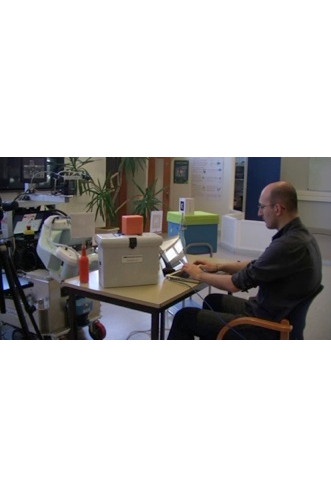
\includegraphics[width=0.2\textwidth]{reachex-1.png} }
%    \subfigure[] {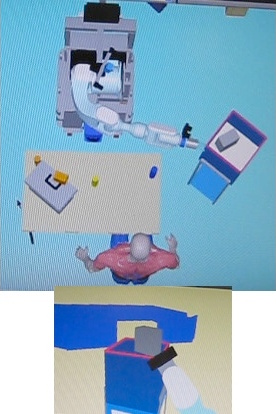
\includegraphics[width=0.2\textwidth]{reachex-2.jpg} }
%    \subfigure[] {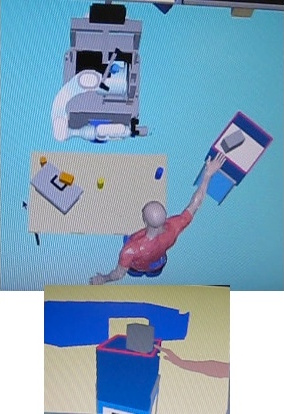
\includegraphics[width=0.2\textwidth]{reachex-3.jpg} }
%    \subfigure[] {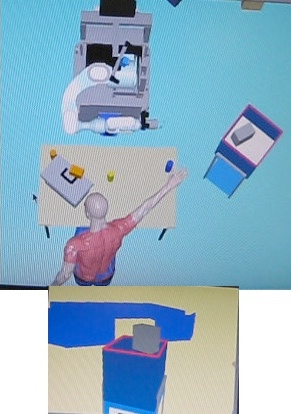
\includegraphics[width=0.2\textwidth]{reachex-4.jpg} }
%    \caption{An example illustrating the \textit{reachable} relation. The
%        relation is computed from the perspectives of both the robot and the
%        human. The computed posture at each step is illustrated with a global
%        view of the scene (top), and from a closest view (bottom). The robot
%        and its human partner are placed face to face (a).  The robot first
%        estimates if the small grey box is reachable to itself using an inverse
%        kinematic (IK) solver and collision checks to find a collision free
%        posture to reach the object (b). Next the robot switches to the human's
%        perspective to estimate if the same object is reachable to the human as
%        well (c).  In the last scene, the human moves towards his left, farther
%        from the object (d). The situation is then reevaluated. In this occasion
%        though, the reasoner cannot find a satisfactory posture for the human to
%    reach the box because he is too far from the target.  }
%
%\label{fig::reach-ex}
%\end{figure*}
%

\paragraph{Hypotheses on Objects States and Positions}

\fxfatal{Rephrase}
It is sometimes difficult or even impossible to see and/or track an object in
certain states. This happens, for instance, when the object is hidden in a
container, when the robot holds it in its gripper, and more generally in any
state in which it is hidden by something else. {\sc Spark} models the possible
symbolic states of objects (whether the object is on a furniture, in an agent
hand, in a container, etc.): According to the robot perception of what has
happened since the object was last seen, the robot builds a belief of the
current possible state with associated probability model.

\subsubsection{Primitive Action Recognition}

Monitoring human activity is crucial for maintaining a coherent state of the
world. Full human action and activity monitoring is a task that requires
knowledge and reasoning both on high level facts like goals, intentions and
plans, as well as bottom-up data from agent and object motions. Simple temporal
and geometric reasoning on human hand trajectories and potential objects
placements can provide some useful clues for high level human monitoring
processes. We call this temporal and geometric reasoning \emph{primitive action
recognition}. Those primitive actions are assessed through monitoring situations
like ``an empty hand is close to an object on a table'' (precursor for a
\emph{pick}), or ``a hand holding an object is over a container'' (precursor for
a \emph{throw}). \emph{Spark} recognises a handful \fxfatal{which ones?} of these
primitives, that are relied on by the robot to track the state transitions in
the human plans (as explained below, at section~\ref{hatp}).

%\subsubsection{Ego-centric and Allo-centric Frames}
%
%{\sc Spark} also supports \emph{perspective-taking}: spatial relations between entities can
%be computed from different viewpoints, which let the robot build for each
%agents it interacts with a different, \emph{perspective-aware} symbolic model
%of the environment. These models are separately stored in the knowledge base.
%
%This allows us to deal with ambiguities that arise when one speaker refers to
%an object within a reference system (or changes the reference system, \ie
%switches perspective) without making the reference frame
%explicit~\cite{Breazeal2006, Ros2010}.
%
%As a result, the robot stores models of the environment either in the
%\emph{ego-centric} reference frame (from the robot perspective) or in 
%\emph{allo-centric} frames (addressee-centred).

\subsubsection{Limitations}

The main weakness of our current implementation relates to the way semantics are
conveyed: because we use 2D markers for artifacts, we skip most of the object
extraction and recognition challenges. Each object has a unique identifier,
which enable us to load a proper CAD model suitable for 3D spatial reasoning
and prevent recognition mistakes in the knowledge base. While {\sc Spark}
algorithms themselves are ignorant of the input sources, and would work equally
well with a full object recognition stack, we do not have tackled it yet.

Besides, temporal reasoning (essential for accurate action recognition for
instance) is not properly addressed in our stack. Temporal reasoning is used
only locally, and does not allow for tracking of long or global events.


%%%%%%%%%%%%%%%%%%%%%%%%%%%%%%%%%%%%%%%%%%%%%%%%%%%%%%%%%%%%%%%%%%%%%%%%%%%%%%%%
\subsection{Multi-modal Communication}
\label{sect|com}

\subsubsection{Natural language grounding}

Natural language processing is one of the fields of human-robot interaction
for which the introduction of the semantic layer has been most beneficial.
In~\cite{Lemaignan2011a} we detail the techniques and the tool called
\texttt{dialogs} that we have developed for natural English language parsing and
grounding, along with verbalisation and (minimalist) dialogue management.

Natural language input (in experiments, we rely on an Android-based interface,
with Google speech recognition) is parsed into a grammatical structure, and
atoms of each sentence are resolved with the help of the ontology to ground
concepts like objects (\ie when a user says ``pick the can'', it resolves to which
instance of \emph{can} the user is referring to) and actions. Sentences are
sorted into questions, desires and statements, and processed accordingly.
Figure~\ref{dialogs|ex} gives a example of the processing of a simple order.

\begin{figure}
    \centering
	\begin{tabular}{l|l}
	\emph{Initial human knowledge} &
	\emph{Human input}\\
	
	\hline
	
    	\stmt{book\_1 type Book} &
	``Give me the book.'' \\
	
    	\stmt{book\_1 hasColor blue} & \\
	\vspace{0.5em}\\
	\hline
    	
	\emph{Generated partial statements} &
	\emph{Newly created statements}\\
	\hline
    	\stmt{?obj type Book} & 
	\stmt{human desires sit\_1} \\
	
	\hspace{0.2cm}$\Rightarrow$ \concept{?obj = book\_1}
    	& \stmt{sit\_1 type Give} \\
    	& \stmt{sit\_1 performedBy myself} \\
    	& \stmt{sit\_1 actsOnObject book\_01} \\
    	& \stmt{sit\_1 receivedBy human} \\
	\end{tabular}

    \caption{Processing an order: this simple example (no ambiguity), taken
    from~\cite{Lemaignan2011a}, shows the thematic roles computed by 
    {\sc Dialogs} for the order ``Give me the book''.}

    \label{dialogs|ex}
\end{figure}


The system supports quantification (``give me \{a | the | some | all | any |
...\} can''), thematic roles (action-specific predicates that qualify the
actions), interactive disambiguation (the robot asks questions when it needs
more information), anaphora resolution (``give \emph{it} to me'') based on
dialogue history. It also permits knowledge extension by learning new semantic
structures (for instance, a sentence like ``learn that cats are animals'' is
converted into \stmt{Cat subClassOf Animal} and added to the knowledge base
after checking for possible contradictions with existing knowledge),
interprets common temporal and place adverbs (like \emph{above} or
\emph{tomorrow}) and translates to a certain extend \emph{states} (``I'm
tired'') into \emph{experiences} (\stmt{HUMAN experiences state\_1, state\_1
hasFeature tired}). We kindly refer the readers to~\cite{Lemaignan2011a} for a
complete discussion of these capabilities and the related algorithms.

\subsubsection{Multi-modal communication}

Because all components rely on the same RDF formalism to format their outputs,
the different communication modalities (\emph{explicit} like verbal, deictic or
based on gaze, or \emph{implicit} like postures) are presented in a homogeneous
way, as statements in the knowledge base. The dialogue grounding process makes
use of them at two distinct levels to provide seamless multi-modal interaction.

First, particular steps of the grounding process explicitly check for the
presence and value of specific facts: for instance, when several instances
match a category (the human says ``give me the bottle'' and the robot knows
about three bottles), the module may decide (it actually depends on the
quantifier preceding the class) to discard some of them based on their
\emph{visibility} for the speaker (implicit communication context built on the
human posture).

Another example, when the human says ``this'', the robot checks if the human is
currently pointing at some object. In that case, \emph{this} is replaced by the
object focused on. Otherwise, the robot performs a lookup in the dialogue history
to find a previous concept that the user could refer to (anaphora resolution).

Note that, while the system benefits from the complementary modalities, they are
not all required. The dialogue system can run with the verbal modality alone, at
the cost of a simpler interaction: if the human says ``this'' without the robot
tracking what the human points at, no \stmt{HUMAN pointsAt ...} fact is
available in the knowledge base, and the robot fallbacks on the anaphora
resolution step alone.

The second level of integration of multi-modality is implicit. By continuously
computing symbolic properties from the geometric model, richer descriptions and
hence discrimination possibilities are available. For instance, the robot may
compute that one bottle is next to a glass while another one stands alone, and
these symbolic descriptions are transparently re-used in a dialogue context to
generate unambiguous references to discriminate between similar objects: ``do
you mean the bottle that is next to the glass?'' (we kindly refer the interested
readers to~\cite{Ros2010b} for a detailed account of our approach to interactive
concept discrimination, along with the related algorithms).

%%%%%%%%%%%%%%%%%%%%%%%%%%%%%%%%%%%%%%%%%%%%%%%%%%%%%%%%%%%%%%%%%%%%%%%%%%%%%%%%

\subsection{Human-Aware Task Planning}
\label{hatp}

Our execution controllers rely on symbolic task planning to convert long-term
desires into a succession of atomic actions. We use in our architecture the
HATP planner (for Human Aware Task Planner~\cite{Alili2008, Alili2009}).  HATP
is a refinement of a Hierarchical Task Network (HTN). As an HTN, it performs an
iterative task decomposition into sub-tasks until reaching atomic actions. The
\emph{planning domain} defines the set of methods describing how to decompose a
task and represents the procedural knowledge of the robot. It is stored outside
of the central knowledge base, using a specific formalism.

\subsubsection{Agents and Action Streams}

HATP originality resides in its ability to produce plans for the robot's actions
\emph{as well as for the other participants} (humans or robots), so-called
\emph{shared plans}. This effectively enriches the robot's interaction
capabilities by allowing for a form of \emph{human behaviour prediction}, which
is used in turn by the robot execution controller to monitor the engagement of
the human partner during joint tasks.

The planner also generates synchronisation points between the agents.
Figure~\ref{plan_hatp1} illustrates such a plan with two streams.  Here, the
robot needs to wait for the success of the human agent's {\tt PUT} action
(estimated through the fulfilment of the action post-conditions, typically
$\neg$\stmt{GREY\_TAPE isOn TABLE}) to be able to start its own action.

We also use shared plans to verbalise the sequence of actions and to explain
the human partner how a task may be shared~\cite{warnier2012when}.

\begin{figure}[htbp]
    \centering
\resizebox{0.9\textwidth}{!}{%
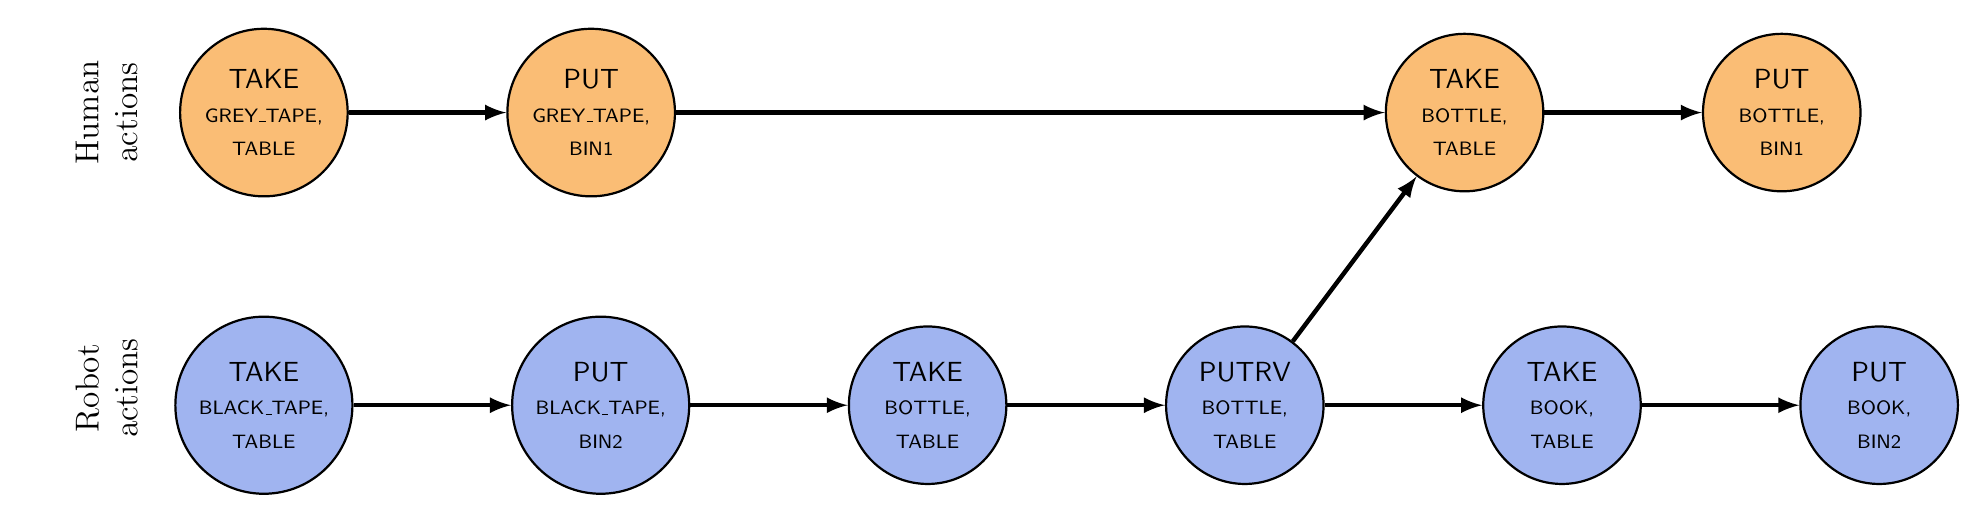
\begin{tikzpicture}[
    >=latex,
    robot/.style={fill=RoyalBlue!50},
    every edge/.style={<-, draw, ultra thick},
    every node/.style={ draw, 
                        thick,  
                        circle, 
                        font=\sf,
                        align=center,
                        node distance=2cm,
                        fill=BurntOrange!50, 
                        minimum size=2cm, 
                        inner sep=0.1cm}]

    \node[font=\rm\large, draw=none, fill=none, rotate=90] at (-2, 0) {Human\\actions};
    \node[font=\rm\large, draw=none, fill=none, rotate=90] at (-2, -3.5) {Robot\\actions};

    \node (h1) {\action{TAKE}{GREY\_TAPE}{TABLE}};
    \node[right=of h1] (h2) {\action{PUT}{GREY\_TAPE}{BIN1 }} edge (h1);

    \node[robot, below=1.5 of h1] (r1) {\action{TAKE}{BLACK\_TAPE}{TABLE }};
    \node[robot, right=of r1] (r2) {\action{PUT}{BLACK\_TAPE}{BIN2 }} edge (r1);
    \node[robot, right=of r2] (r3) {\action{TAKE}{BOTTLE}{TABLE }} edge (r2);
    \node[robot, right=of r3] (r4) {\action{PUTRV}{BOTTLE}{TABLE}} edge (r3);
    \node[robot, right=of r4] (r5) {\action{TAKE}{BOOK}{TABLE }} edge (r4);
    \node[robot, right=of r5] (r6) {\action{PUT}{BOOK}{BIN2 }} edge (r5);

    \node[right=9cm of h2] (h3) {\action{TAKE}{BOTTLE}{TABLE}} edge (h2) edge (r4);
    \node[right=of h3] (h4) {\action{PUT}{BOTTLE}{BIN1}} edge (h3);

\end{tikzpicture}
}
\caption{A plan produced by HATP with two action streams (here, human actions
    are at the top while robot actions are at the bottom). The arrow between the
    two streams represents a synchronization point ({\sf PUTRV} stands for {\it Put it so it is both
    reachable and visible}).}

  \label{plan_hatp1}
\end{figure}

\subsubsection{Action Costs and Social Rules}

A cost and a duration function is associated to each action.  The duration
function provides a duration interval for the action achievement and is used, in
one hand, to schedule the different streams and, in the other hand, as an
additional cost function.

In addition to these costs, HATP also takes into
account a set of social rules.  Social rules are constraints aiming at leading
the plan construction towards the best plan according to some human preferences.
The social rules we have defined so far deal with:

\begin{itemize}
\item undesirable state: to avoid a state in which the human could
  feel uncomfortable;
\item undesirable sequence: to eliminate sequences of actions that can
  be misinterpreted by the human;
\item effort balancing: to adjust the work effort of the agents;
\item wasted time: used to avoid long delays between the actions of
  the human partner;
\item intricate links: to limit dependencies between the actions of
  two or more agents.
\end{itemize}

\begin{figure}[htbp]
  \centering
\resizebox{0.9\textwidth}{!}{%
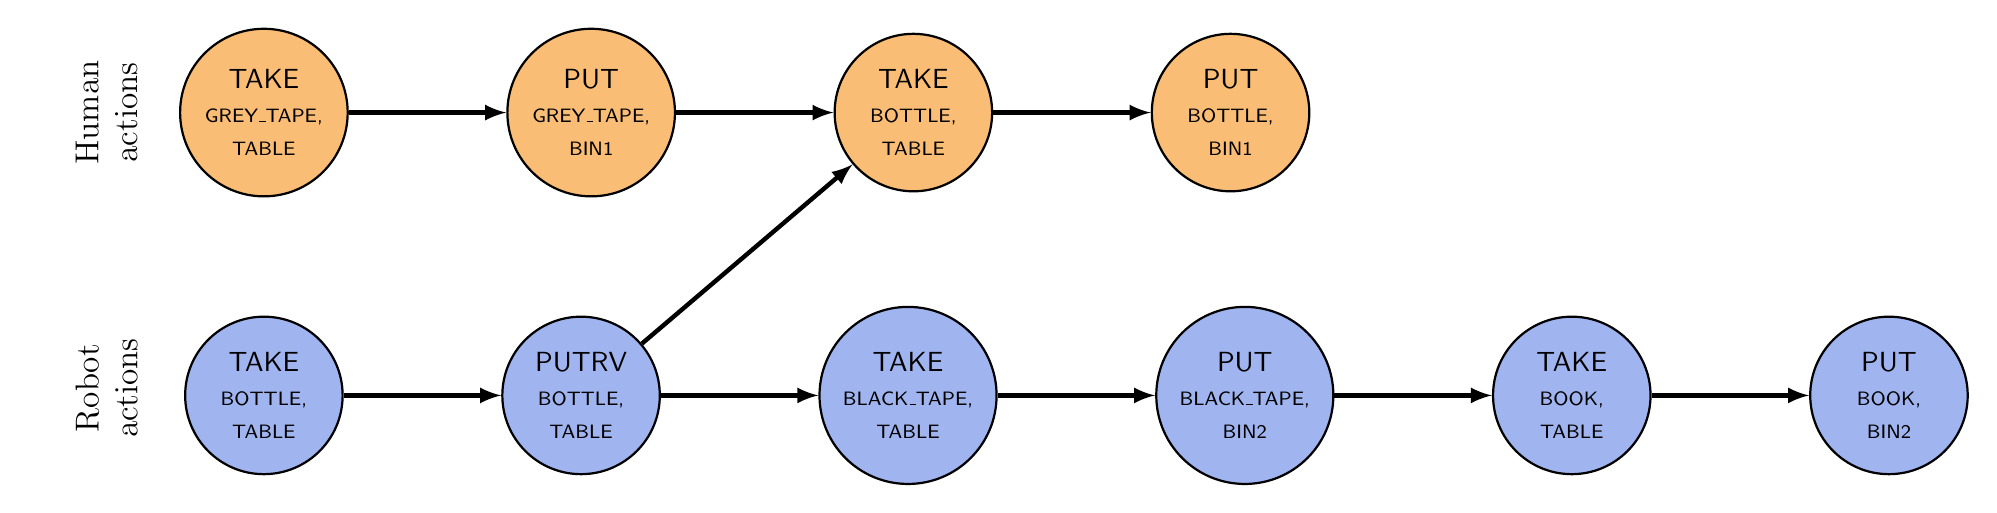
\begin{tikzpicture}[
    >=latex,
    robot/.style={fill=RoyalBlue!50},
    every edge/.style={<-, draw, ultra thick},
    every node/.style={ draw, 
                        thick,  
                        circle, 
                        font=\sf,
                        align=center,
                        node distance=2cm,
                        fill=BurntOrange!50, 
                        minimum size=2cm, 
                        inner sep=0.1cm}]

    \node[font=\rm\large, draw=none, fill=none, rotate=90] at (-2, 0) {Human\\actions};
    \node[font=\rm\large, draw=none, fill=none, rotate=90] at (-2, -3.5) {Robot\\actions};


    \node (h1) {\action{TAKE}{GREY\_TAPE}{TABLE}};
    \node[right=of h1] (h2) {\action{PUT}{GREY\_TAPE}{BIN1 }} edge (h1);

    \node[robot, below=1.5 of h1] (r3) {\action{TAKE}{BOTTLE}{TABLE }};
    \node[robot, right=of r3] (r4) {\action{PUTRV}{BOTTLE}{TABLE}} edge (r3);
    \node[robot, right=of r4] (r1) {\action{TAKE}{BLACK\_TAPE}{TABLE }} edge (r4);
    \node[robot, right=of r1] (r2) {\action{PUT}{BLACK\_TAPE}{BIN2 }} edge (r1);
    \node[robot, right=of r2] (r5) {\action{TAKE}{BOOK}{TABLE }} edge (r2);
    \node[robot, right=of r5] (r6) {\action{PUT}{BOOK}{BIN2 }} edge (r5);

    \node[right=of h2] (h3) {\action{TAKE}{BOTTLE}{TABLE}} edge (h2) edge (r4);
    \node[right=of h3] (h4) {\action{PUT}{BOTTLE}{BIN1}} edge (h3);

\end{tikzpicture}
}

\caption{An alternative plan where the \emph{wasted time} social rule is used to optimise the
total duration of the task. }

  \label{plan_hatp2}
\end{figure}

Figure~\ref{plan_hatp2} illustrates an alternative plan to the previous 
one (Figure~\ref{plan_hatp1}) if the wasted time social rule is used.
The obtained shared plan is the best plan according to a global evaluation of
these multiple criteria.

\subsubsection{Commitment Levels}

By tuning its costs and adapting its social rules, HATP can be used to compute
various alternative plans. These plans can be categorised into several levels of
cooperation

\begin{itemize}
\item helping the human to achieve his goal by acting for him
\item sharing concrete resources by handing some objects
\item collaboration of the robot and the human by coordinating their
  actions towards a human-robot joint goal.
\end{itemize}


Because HATP is a generic symbolic task planner, we have been able to design a
planning domain at a semantic level which is close to the one used in the
human-robot dialogue (the planner vocabulary contains concepts like
\texttt{give}, \texttt{table}, \texttt{is on}...). Hence only a few ontology
rules have been required to map both the knowledge extracted from the situation
assessment and the statements originated from the verbal interaction to the
planner domain.

Also, we would like to mention that, after some research (see appendix B
of~\cite{Lemaignan2012a} for a detailed discussion)  we have decided to
represent neither the planning domain nor the resulting plans in the knowledge
base: the planning domain (with task pre- and postconditions) is stored in a
specific format, outside of the central declarative knowledge repository, and
the plans are directly communicated to the robot controller. Thus, like other
cognitive architectures, we have independent declarative and procedural
knowledge stores.


%%%%%%%%%%%%%%%%%%%%%%%%%%%%%%%%%%%%%%%%%%%%%%%%%%%%%%%%%%%%%%%%%%%%%%%%%%%%%%%%
\subsection{Robot control}
\label{sect|ctrl}

While parts of the architecture ({\sc Spark}, {\sc Oro}) have been deployed with external
execution controllers (like {\sc Cram}~\cite{Beetz2010} or the BERT
platform~\cite{Lallee2010b}, as reported in~\cite{Lemaignan2010}), we have also
developed dedicated robot controllers which integrate the whole stack introduced
in Figure~\ref{fig|archi}. {\sc Shary}~\cite{clodic2008shary} is the main one,
written in the PRS~\cite{Ingrand1996} language. We also use the Python-based
{\sc pyRobots} collection of tools that provide a large set of high-level
actions and an event-based architecture well suited for prototyping.
They both rely on deep integration with the knowledge base that serves as the
primary source of semantics for decision making.

The novelty of our contribution here is the interleaving of a semantic-aware
architecture designed for autonomy with human-aware decisional components. To
our knowledge, no other robotic architecture covers in depth those two
perspectives.

The Ke Jia project~\cite{Chen2010} is maybe one of the closest
approach. It integrates on a mobile platform a knowledge representation language
with natural language processing, task planning and motion planning. Default and
non-monotonic reasoning has been especially researched within the Ke Jia project
for symbolic task planning~\cite{Ji2011} and underspecified natural language
processing. The Ke Jia robot has been demonstrated in several tasks involving human-robot
interaction with natural language. These tasks include a task with multiple
\emph{pick \& carry} that are globally optimised, naive physics reasoning via
taught rules or more complex scenarios with the robot delivering drinks, taking
into account changing and mutually exclusive preferences of users.

Also notable, Beetz et al.~\cite{Beetz2010} proposes a cognitive architecture
called \textsc{CRAM} (Cognitive Robot Abstract Machine) that deeply integrates
with \textsc{KnowRob}~\cite{Tenorth2009a}, a knowledge processing framework
based on Prolog. Its underlying storage is based on an OWL ontology, derived
from \textsc{OpenCyc}. \textsc{CRAM} and \textsc{KnowRob} have been demonstrated
on several real-world scenarios, where natural language recipes extracted from
the Internet had to be translated into plans and executed in a kitchen
environment, perceived and rebuilt on-line by the robots. This architecture has
however not been deployed in many scenarios involving human-robot interactions.


\subsubsection{Desires and experiences}

We split the interaction situations stemming from the situation assessment and
communication components in two categories: \emph{desires} (related to
\emph{performative acts} in Austin's classification of speech
acts~\cite{Austin1962}) and \emph{experiences}.

\emph{Desires} are typically human orders (``Give me that book''). The nature
of the desired action (to pick, give, look, bring, show...), along with the
action parametrization (what is acted on? who should perform the action? etc.)
are extracted from the knowledge base, and either passed to a task planner
(presented in the previous section) or executed if the procedure is directly
available.

\emph{Experiences}, on the other hand, comprise of emotions, states and
questions (when asking a question, we consider the human to be in an
\emph{interrogative state}). When the knowledge base states that an agent
\emph{experiences} a particular emotion or state, the execution controller may
decide to handle it, typically by trying to answer the question or using the
emotional or physical state as a parameter for subsequent actions. As an
example, when the speaker says ``I feel tired'', we change the motion planner
parametrization to lower the effort the human needs to provide for the following
joint manipulation tasks.\footnote{Note that this very example has been
implemented as a proof-of-concept. A broader framework that would support
action alteration based on the user's experienced states remains to be worked on.}

\subsubsection{Event-driven control}

The {\sc Oro} server proposes two paradigms to access its content: RPC-style
queries (based on the standard SPARQL language) or events. A module can
subscribe to an event by passing through an event pattern (in its simplest
form, a partial statement like \stmt{? type Elephant}) and a callback.  Each
time a new instance of elephant appears in the knowledge base, the callback is
triggered.

This allows us to write reactive robot controllers with a high level of
expressiveness: for instance, by subscribing to the event \stmt{human1 desires
?action, ?action type Look, ?action hasGoal myself}, we could trigger a
behaviour when the human expresses (through dialogue, gestures...) that he
wants to look at the robot itself.

The robot controller designer does not need to directly care about how this
\emph{desire} is produced (this is delegated to perception modules), he can
focus on the semantic of the desire.

Note also that we take advantage of the reasoning capabilities of the system:
for example, the goal of the action (\stmt{action hasGoal myself}) may not be
explicitly asserted, but inferred by the reasoner based on other assertions.

\subsubsection{Action Execution and Monitoring}\label{sec:action}

Action execution and monitoring is the central activity of the robot executive
controller, and involves interaction with most of the components presented on
Figure~\ref{fig|archi}.

Like most robotic architecture, actions are split into \emph{atomic actions}
and more complex \emph{tasks}. Tasks are created either statically or dynamically.
The {\sc pyRobots} controller, for instance, combines the actions listed in
table~\ref{table|pyrobots_actions} to implement the high-level tasks it exposes: {\tt
lookAt}, {\tt moveTo}, {\tt getFromHuman}, {\tt showObject}, {\tt giveObject},
{\tt pickObject}, {\tt bringObject}, {\tt putObject}, {\tt hideObject}.

Our other controller, {\sc Shary}, relies on the symbolic task planner to
generate at run-time suitable sets of atomic actions.

\begin{table}[ht!]
\begin{center}
\begin{tabular}{p{0.8\columnwidth}}
\hline
    {\bf Manipulation} \\
     {\tt attachobject}, {\tt basicgive}, {\tt basictake}, {\tt close\_gripper}, {\tt configure\_grippers}, {\tt grab\_gripper}, {\tt handover}, {\tt hide}, {\tt open\_gripper}, {\tt pick}, {\tt put}, {\tt put\_accessible}, {\tt release\_gripper}, {\tt show}, {\tt take} \\
\hline
    {\bf Gaze control} \\
     {\tt glance\_to}, {\tt look\_at}, {\tt sweep}, {\tt switch\_active\_stereo\_pair}, {\tt track}, {\tt cancel\_track} \\
\hline
    {\bf Navigation} \\
     {\tt carry}, {\tt follow}, {\tt cancel\_follow}, {\tt goto}, {\tt moveclose}, {\tt waypoints} \\
\hline
    {\bf Local navigation} \\
     {\tt dock}, {\tt rotate}, {\tt translate} \\
\hline
    {\bf Posture configuration} \\
     {\tt extractpose}, {\tt idle}, {\tt manipose}, {\tt movearm}, {\tt rest}, {\tt setpose}, {\tt settorso}, {\tt tuckedpose} \\
\hline
\end{tabular}
\end{center}
\caption{Main {\sc pyRobots} \emph{actions}, sorted by categories. These
actions are combined at run-time into higher-level \emph{tasks}.}

\label{table|pyrobots_actions}
\end{table}

\paragraph{Human-Aware Motion, Placement and Manipulation Planning}
Manipulation and navigation actions listed in
table~\ref{table|pyrobots_actions} rely on a collection of dedicated 3D motion
planner to generate movements that are aware of surrounding humans. Robot
placement and end-effectors trajectories are computed on-line to allow object
manipulation that take into account task specific constraints and human
postures, abilities and preferences. \cite{Sisbot2008, Mainprice2011,
Pandey2011} detail these techniques.


\paragraph{Action Execution and Monitoring Robot Controller}
Based on context and on the shared plan elaborated by HATP for a given goal,
the robot controller decides to execute an action or to ask its human
partner to do it.  Actions feasibility by the human or the robot are
regularly reconsidered based on the reachability / visibility
computation mechanisms.

Robot action execution is based on simple automatons  that translate
symbolic planning atomic actions into sequences of planned arm motions
and gripper commands to execute according to current state
of the 3-tuple (gripper, object, furniture). We have three states
according to whether the object is in gripper and if it is in gripper
whether it is on furniture.  These states are directly obtained from
the updated symbolic state of the world in the ontology.

For plan action monitoring, primitive actions recognition is used. A primitive
action detection is interpreted as action success if it is the expected one and
failure otherwise. The robot also reacts to the absence of activity.



%%%%%%%%%%%%%%%%%%%%%%%%%%%%%%%%%%%%%%%%%%%%%%%%%%%%%%%%%%%%%%%%%%%%%%%%%%%%%%%%
%%%%%%%%%%%%%%%%%%%%%%%%%%%%%%%%%%%%%%%%%%%%%%%%%%%%%%%%%%%%%%%%%%%%%%%%%%%%%%%%
%%%%%%%%%%%%%%%%%%%%%%%%%%%%%%%%%%%%%%%%%%%%%%%%%%%%%%%%%%%%%%%%%%%%%%%%%%%%%%%%

\section{Support Studies}
\label{sec:expe}

Our architecture has been deployed and tested in a number of studies on
several robotic platforms. Table~\ref{table|experiences} lists the most
significant ones, with their main focuses and reference publications.

\begin{table*}
\begin{center}

\begin{tabular}{lll}
 \bf{Study} & Focus & Reference \\
\hline
{\it Point \& Learn} (2010) & Interactive knowledge acquisition & \cite{Lemaignan2010} \\
{\it Spy Game} (2010) & Interactive object discrimination & \cite{Ros2010b} \\
{\it Interactive Grounding I} (2011) & Multi-modal interaction, perspective taking & \cite{lemaignan2011what} \\
{\it Roboscopie} (2011) & Theater, reflection on the future of HRI & \cite{lemaignan2012roboscopie} \\
{\it Cleaning the table} (2011) & Whole stack integration & \cite{Alami2011} \\
{\it I'm in your shoes} (2012) & False beliefs & \cite{warnier2012when} \\
{\it Give me this} (2012) & Natural joint object manipulation & \cite{gharbi2013natural} \\
{\it Interactive Grounding II} (2012) & Multi-modal interaction, perspective taking & \cite{lemaignan2013talking} \\
\hline

\end{tabular}
\end{center}
\caption{Main studies conducted with our cognitive architecture.}
\label{table|experiments}
\end{table*}

We briefly introduce two of them in order to illustrate in a practical way
different aspects of the architecture that were previously presented.  The first
one is focused on knowledge representation and verbal interaction: the human
asks for help to find and pack objects ({\it Interactive Grounding I} in
Table~\ref{table|experiments}). The second one ({\it Cleaning the table})
involves the {\sc Shary} execution controller and the HATP symbolic task planner
besides {\sc Oro} and {\sc Dialogs}. In this scenario, the human and the robot
try to cooperatively remove objects from a table, and behaviours and motions are
fully planned and executed.

\subsection{Interactive Grounding}
\label{moving-london}

This first study is based on the following scenario: Tom and Jerry are moving to
London, so they are packing things in boxes. \emph{Jido}, a dual-arm
manipulator, is observing while they move things here and there
(Figure~\ref{fig|vpt}).  They ask questions to Jido to know where certain
objects are located (\emph{Where is the white tape? What is behind the toolbox?}
etc.). This study focuses on multi-modal ,interactive grounding only, and
the robot does not perform any action.

Objects are perceived solely through 2D fiducial markers sticked on them, and humans are
tracked through motion capture. The robot knowledge base is initialised with
the {\sc Oro} commonsense ontology.  We next describe two
situations where we can follow the internal robot's reasoning and the
interaction with the users.

\paragraph{Implicit Disambiguation Through Visual Perspective Taking}

\begin{figure}[!ht]
  \centering
  \subfigure [Interactive grounding in a cluttered environment.]{
  \label{fig|vpt}
  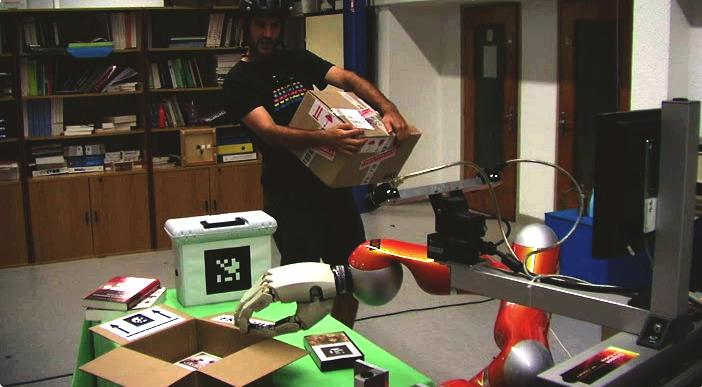
\includegraphics[width=0.48\linewidth]{pt.jpg}
}%
\subfigure [Disambiguation through pointing.]{
  \label{fig|pointing}
  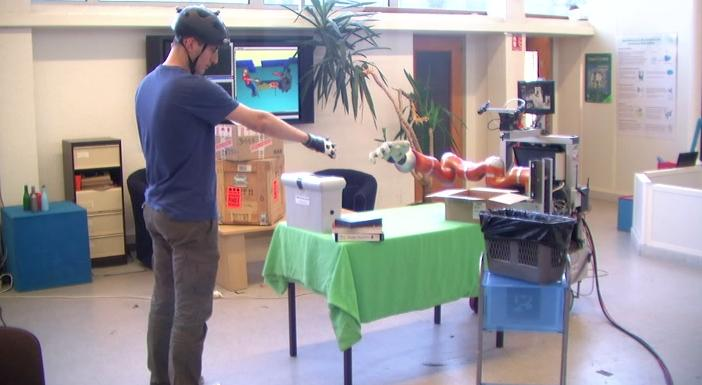
\includegraphics[width=0.48\linewidth]{inTheBox2.jpg}
}
\end{figure}


Tom enters the room while carrying a big box (Figure~\ref{fig|vpt}). He
approaches the table and asks Jido to hand him the video tape: ``Jido, can
you give me the video tape''. The \textsc{Dialogs} module processes this
sentence, and queries the ontology to
identify the object the human is referring to: \stmt{?obj type VideoTape}. 

There are two video tapes in the scene: one on the table, and another one
inside the cardboard box. Thus, the knowledge base returns both: $\Rightarrow$
\concept{?obj = [videoTape1, videoTape2]}. 

However, only one is visible for Tom (the one on the table). Although there is
an ambiguity from the robot's perspective, the human referred to the tape using
the definite article \emph{the}: this is interpreted by the natural language
processor as the human referring to a precise object, in that case, the visible
one.\footnote{Other heuristics are available to the {\sc Dialogs} module: for
instance, if a tape had been recently mentioned in the dialogue, this instance
would have been selected instead as the referent.}

%Since only one object remains (\ie the referent that \concept{VideoTape} stands
%for is not ambiguous any more), the robot infers that the human refers to it and
%eventually execute the command, \ie give it to the human. Alternatively, the
%robot first asks the human for confirmation (``was \concept{videoTape1} the
%object you had in mind?'') before proceeding with the action.
%Table~\ref{table|ptbeliefs} lists the robot's beliefs about itself and its human
%partner involved in this situation.
%
%\begin{table}[ht!]
%\begin{center}
%    \subfigure{
%\begin{tabular}{l}
%\hline
%Robot's beliefs about itself (\emph{robot's model}):\\
%\hline
%  \hspace{0.7cm}\stmt{videoTape1 type VideoTape}\\
%  \hspace{0.7cm}\stmt{videoTape1 isOn table}\\
%  \hspace{0.7cm}\stmt{videoTape1 isVisible true}\\
%  \hspace{0.7cm}\stmt{videoTape2 type VideoTape}\\
%  \hspace{0.7cm}\stmt{videoTape2 isIn cardBoardBox}\\
%  \hspace{0.7cm}\stmt{videoTape2 isVisible true}\\
%\hline
%\end{tabular}
%}\hspace{1em}%
%    \subfigure{
%\begin{tabular}{l}
%\hline
%Robot's beliefs about Tom (\emph{Tom's model}):\\
%\hline
%  \hspace{0.7cm}\stmt{videoTape1 type VideoTape}\\
%  \hspace{0.7cm}\stmt{videoTape1 isOn table}\\
%  \hspace{0.7cm}\stmt{videoTape1 isVisible true}\\
%  \hspace{0.7cm}\stmt{videoTape2 type VideoTape}\\
%  \hspace{0.7cm}\stmt{videoTape2 isIn cardBoardBox}\\
%  \hspace{0.7cm}\stmt{videoTape2 isVisible false}\\
% \hline
%\end{tabular}
%}
%\end{center}
%\caption{Robot's beliefs about itself and its human partner.}
%\label{table|ptbeliefs}
%\end{table}
%
\paragraph{Explicit Disambiguation Through Verbal Interaction and Gestures}

In this second situation, Jerry enters the living room without knowing where Tom had
placed the video tapes (Figure~\ref{fig|pointing}). So he first asks Jido:
``What's in the box?''. Before the robot can answer the question it has to
figure out which box Jerry is talking about. Similar to the previous situation,
two boxes are visible: 

\begin{center}
\begin{tabular}{l}
\stmt{?obj type box}\\
\hspace{0.7cm}$\Rightarrow$ {\tt ?obj = [cardBoardBox, toolbox]}
\end{tabular}
\end{center}

However both are also visible to the human and the previous ambiguity resolution
procedure can not be applied. The robot generates a question (using the
\emph{Discrimination} algorithm that we introduced at section~\ref{reasoning})
and asks Jerry which box he is referring to: ``Which box, the toolbox or the
cardboard box?'' Jerry can answer the question, but he instead decides to point
at it: ``This box'' (Figure~\ref{fig|pointing}). {\sc Spark} identifies the {\tt
cardBoardBox} as being pointed at and looked at by the human and updates the
ontology with this new information using a rule available in the common-sense
ontology \stmt{pointsAt(?ag, ?obj) $\land$ looksAt(?ag, ?obj) $\to$
focusesOn(?ag, ?obj)}. The \textsc{Dialogs} module is then able to merge both
sources of information, verbal (``this'') and deictic to distinguish the box
Jerry refers to:

\begin{center} 
    \begin{tabular}{l} 
        \stmt{Jerry pointsAt carboardBox}\\ 
        \stmt{Jerry looksAt carboardBox}\\ 
        $\to$ \stmt{Jerry focusesAt carboardBox}\\ 
        \hspace{0.7cm}$\Rightarrow$ {\tt ?obj = [cardBoardBox]}
    \end{tabular} 
\end{center}

Finally, the \textsc{Dialogs} queries the ontology about the content of the box
and the question can be answered: ``Wall-E'' (the label of the object, stored in the
ontology, is used to interact with the user).

%\begin{center}
%\stmt{?obj isIn cardBoardBox}\\
%\hspace{0.7cm}$\Rightarrow$ \concept{?obj = videoTape2}\\
%\end{center}

At this point Jerry wants to know where is the other tape: ``And where is the
other tape?''. \textsc{Dialogs} processes this sentence using the
\concept{differentFrom} OWL predicate:

\begin{center}
\begin{tabular}{l}
\stmt{?obj type VideoTape}\\
\stmt{?obj differentFrom videoTape2}\\
\hspace{0.7cm}$\Rightarrow$ \concept{?obj = [videoTape1]}
\end{tabular}
\end{center}

Since there is only one possible ``other'' video, no specific disambiguation is
required, and the robot verbalises the result of the query to the knowledge
base: ``The other tape is on the table and next to the toolbox.''

\begin{center}
\begin{tabular}{l}
\stmt{videoTape1 isOn table}\\
\stmt{videoTape1 isNextTo toolbox}
\end{tabular}
\end{center}


\subsection{\emph{Cleaning the table} study}

\begin{figure}[ht!]
    \centering
    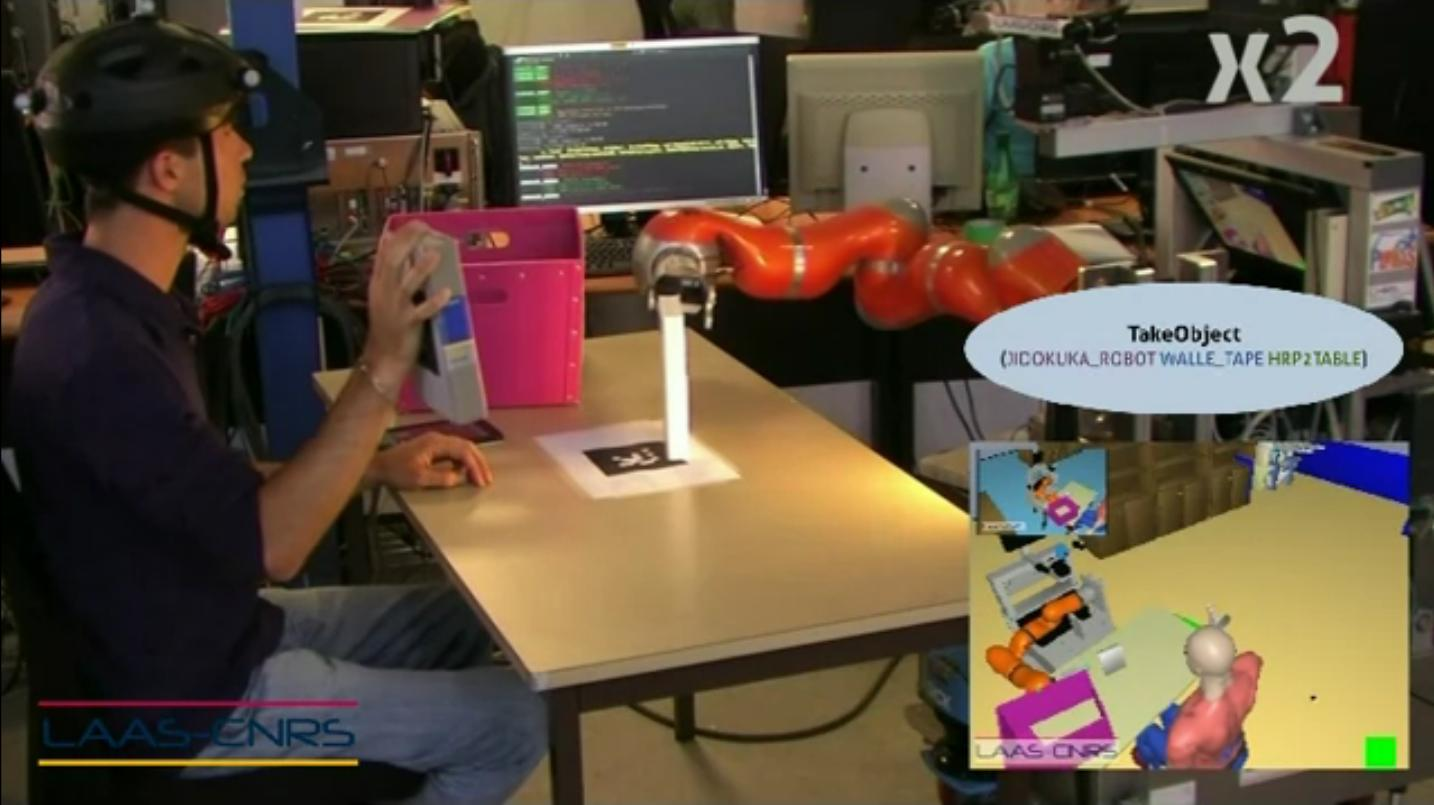
\includegraphics[width=0.6\columnwidth]{cleantable.jpg}

    \caption{Face-to-face setting of the \emph{Clean the Table} scenario. The
    physical situation, the {\sc Spark} model, and the current step of the plan
    are visible on the picture.}

    \label{fig|cleantable-video}
\end{figure}


This study demonstrates a richer decision-making process. The {\sc Oro} server
is used in conjunction with the HATP symbolic task planner and the {\sc Shary}
execution controller to produce and execute a shared plan.

%In this scenario (Figure~\ref{fig|cleantable-video}), a human and a robot
%cooperate to remove objects from a table. The robot produces symbolic plans for
%both itself and the human (Figure~\ref{plan-etat2})
%that allow the robot to (verbally) share the task with the human (like ``I take
%the green box and I put it in the trashbin, you take the black video tape and
%you throw it in the trashbin''). Plans are created based on perceived
%visibility and reachability of the objects, and the robot also monitors the
%human activities to track the advancement of the whole plan.

%
%\begin{figure*}[thpb]
%  \centering
%\resizebox{0.9\textwidth}{!}{%
%\begin{tikzpicture}[
%    >=latex,
%    robot/.style={fill=RoyalBlue!50},
%    every edge/.style={<-, draw, ultra thick},
%    every node/.style={ draw, 
%                        thick,  
%                        circle, 
%                        font=\sf,
%                        align=center,
%                        node distance=2cm,
%                        fill=BurntOrange!50, 
%                        minimum size=2cm, 
%                        inner sep=0.1cm}]
%
%    \node[font=\rm\large, draw=none, fill=none, rotate=90] at (-2, 0) {Human\\actions};
%    \node[font=\rm\large, draw=none, fill=none, rotate=90] at (-2, -3.5) {Robot\\actions};
%
%
%    \node (h1) {\action{TAKE}{WALLE\_TAPE}{TABLE}};
%    \node[right=of h1] (h2) {\action{THROW}{WALLE\_TAPE}{TRASH\_1 }} edge (h1);
%
%    \node[robot, below=1.5 of h1] (r1) {\action{TAKE}{GREY\_TAPE}{TABLE }};
%    \node[robot, right=of r1] (r2) {\action{PUTRV}{GREY\_TAPE}{TABLE}} edge (r1);
%    \node[robot, right=of r2] (r3) {\action{TAKE}{LOTR\_TAPE}{TABLE }} edge (r2);
%    \node[robot, right=of r3] (r4) {\action{PUTRV}{LOTR\_TAPE}{TABLE }} edge (r3);
%
%    \node[right=of h2] (h3) {\action{TAKE}{GREY\_TAPE}{TABLE}} edge (h2) edge (r2);
%    \node[right=of h3] (h4) {\action{THROW}{GREY\_TAPE}{TRASH\_1}} edge (h3);
%    \node[right=of h4] (h5) {\action{TAKE}{LOTR\_TAPE}{TABLE}} edge (h4) edge (r4);
%    \node[right=of h5] (h6) {\action{THROW}{LOTR\_TAPE}{TRASH\_1}} edge (h5);
%
%
%\end{tikzpicture}
%}
%
%  \caption {A plan produced by HATP to execute the high-level order ``clean the
%  table''. Two streams of actions are generated: for the human (top) and for the
%  robot (bottom). Synchronization points ensure the coordination.}
%
%  \label{plan-etat2}
%\end{figure*}
%
Figure~\ref{fig|cleantable-timeline} presents a practical sample of the whole
task. It depicts a run with a single tape on a table. The tape is
reachable by the robot only, while the bin where objects are supposed to be
placed is reachable by the human only: the robot needs to come up with a shared
plan that involves joint actions.

The goal is first received by the execution controller (after processing of the
user request by the {\sc Dialogs} module, not shown on the figure). At
$t_1$, the tape is computed by the robot as being reachable by the robot only
(columns \emph{Perception} and \emph{Knowledge}), and the execution controller
invokes the task planner, which produces a joint plan (column \emph{Plan}).

The first task ({\tt TAKE(GREY\_TAPE, TABLE)}) is instantiated by calling the 3D
motion planner (column \emph{Actions}, left). The motion planner returns two atomic
actions ({\tt PICK\_GOTO} followed by {\tt TAKE\_TO\_FREE}) that the controller
executes (by first reaching the object, grasping it and bringing it back to a
free position).  Once the robot's perception allows the controller to ensure
that the task's post-conditions are fulfilled (at $t_2$, by satisfying the
statement \stmt{ROBOT hasInHand TAPE}), the next task is started (placing the
tape so that it becomes reachable by the human).

At $t_3$, the tape is now reachable by the human, and the next tasks (taking the
tape and placing it in the bin) have to be performed by the human: the robot
instructs the user to do so (not pictured on the figure) and monitors the
actions of the human to detect when the tasks' post-conditions are satisfied
(column \emph{Actions}, right). When these post-conditions are fulfilled, the
goal is considered to be completed.

This simple example illustrates how the symbolic facts are produced from the
situation assessment, and, in parallel, used by the execution controller to
assess the overall progress of the plan.

\begin{figure*}[thpb]
  \centering

\renewcommand{\stmt}[1]{{\footnotesize \tt  #1}}
\resizebox{\textwidth}{!}{%
\begin{tikzpicture}[
        >=latex,
        box/.style={draw,rectangle, dotted, minimum width=#1, minimum height=3.8cm},
        box/.default={4.5cm},
        every edge/.style={draw, ultra thick, ->},
        every node/.style={align=center},
        robot/.style={fill=RoyalBlue!50},
        plan/.style={draw,
                     thick,  
                     circle, 
                     font=\sf,
                     align=center,
                     fill=BurntOrange!50, 
                     minimum size=1cm, 
                     inner sep=0.1cm}]


        \coordinate (figbottom) at (-0.5, -28.5);

        \path (-0.5,0) edge (figbottom) node[sloped, above left, rotate=90] {time};

        \node at (2,0) (percept) {\bf Perception};
            \node[below=0.5 of percept.south west, anchor=mid] {camera};
            \node[below=0.5 of percept.south east, anchor=mid] {3D model};
        \node[right=4 of percept, minimum width=2.5cm] (kb) {\bf Knowledge};
            \node[below=0.5 of kb.south west, anchor=mid east] (kbr) {robot};
            \node[below=0.5 of kb.south east, anchor=mid west] (kbh) {human};
            \draw[dotted] (kb.south) to (figbottom -| kb);
        \node[right=4 of kb] (plan) {\bf Plan};
            \node[below=0.5 of plan.south west, anchor=mid east] (probot) {robot};
            \node[below=0.5 of plan.south east, anchor=mid west] (phuman) {human};
        \node[right=5 of plan] (action) {\bf Actions};
            \node[below=0.5 of action.south west, anchor=mid east] (arobot) {robot};
            \node[below=0.5 of action.south east, anchor=west] (ahuman) {human\\(monitoring)};

        \draw[dashed] (-0.6,-1.2) --(24, -1.2);

        \node[anchor=east] at (-0.5, -3) (t1) {$t_1$};
        \node[anchor=east, below=6 of t1] (t2) {$t_2$};
        \node[anchor=east, below=6 of t2] (t3) {$t_3$};
        \node[anchor=east, below=4 of t3] (t4) {$t_4$};
        \node[anchor=east, below=5 of t4] (t5) {$t_5$};

        %%%%%%%%%%%%%%%%%%%%%%%%%%%%%%%%%%%%%%%%%%%%%%%%%%%%%%%%%%%%%%%%%%%%%%%%%%%%%%%%%%%%%%%%%%%%
        %%% PERCEPTIONS
        %%%%%%%%%%%%%%%%%%%%%%%%%%%%%%%%%%%%%%%%%%%%%%%%%%%%%%%%%%%%%%%%%%%%%%%%%%%%%%%%%%%%%%%%%%%%

        \node at (t1 -| percept) (cam1) {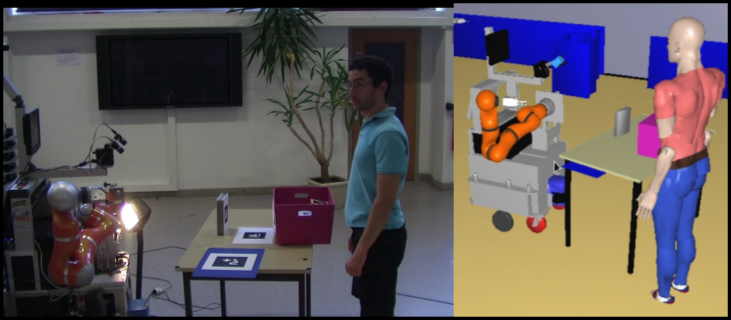
\includegraphics[height=2cm]{manip_run_cam1.png}};
        \node at (t2 -| percept) (cam2) {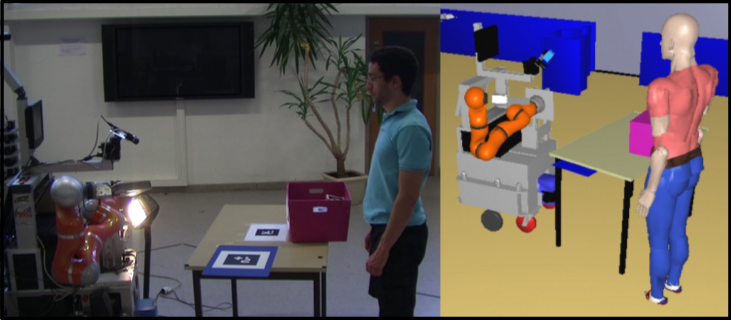
\includegraphics[height=2cm]{manip_run_cam2.png}};
        \node at (t3 -| percept) (cam3) {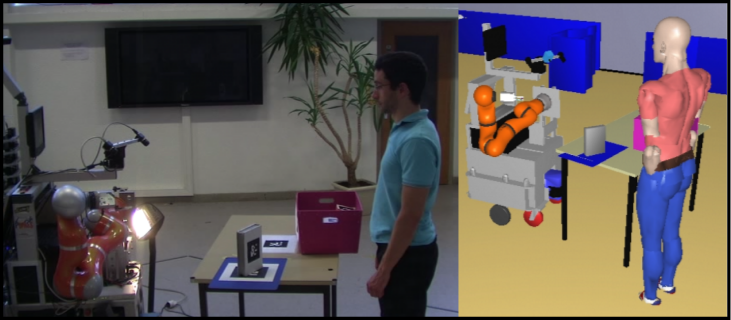
\includegraphics[height=2cm]{manip_run_cam3.png}};
        \node at (t4 -| percept) (cam4) {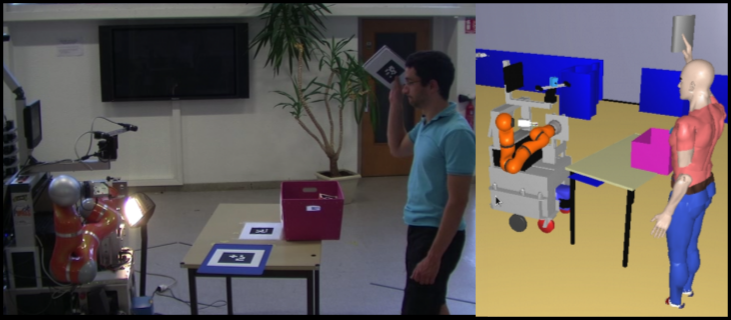
\includegraphics[height=2cm]{manip_run_cam4.png}};
        \node at (t5 -| percept) (cam5) {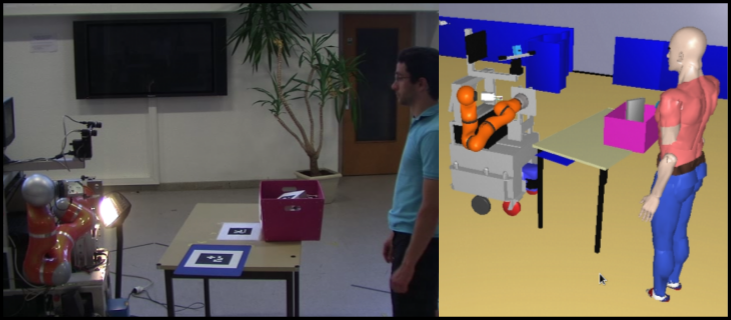
\includegraphics[height=2cm]{manip_run_cam5.png}};

        %%%%%%%%%%%%%%%%%%%%%%%%%%%%%%%%%%%%%%%%%%%%%%%%%%%%%%%%%%%%%%%%%%%%%%%%%%%%%%%%%%%%%%%%%%%%
        %%% KNOWLEDGE
        %%%%%%%%%%%%%%%%%%%%%%%%%%%%%%%%%%%%%%%%%%%%%%%%%%%%%%%%%%%%%%%%%%%%%%%%%%%%%%%%%%%%%%%%%%%%

        \node[align=left] at (cam1 -| kbr) (kb1) {\stmt{TAPE isReachable true}\\
                                                        \stmt{TAPE isVisible true} \\
                                                        \stmt{TAPE isOn TABLE}};

        \node[align=left] at (cam1 -| kbh) {\stmt{TAPE isReachable false}\\
                                                        \stmt{TAPE isVisible true}};

        \node[align=left] at (cam2 -| kbr) (kb2) {\stmt{ROBOT hasInHand TAPE}};


        \node[align=left] at (cam3 -| kbr) {\stmt{TAPE isReachable true}\\
                                            \stmt{TAPE isVisible true} \\
                                            \stmt{TAPE isOn TABLE}};

        \node[align=left ] at (cam3 -| kbh) (kb3) {\stmt{TAPE isReachable true}\\
                                             \stmt{TAPE isVisible true}};

        \node[align=left] at (cam4 -| kbh) (kb4) {\stmt{HUMAN hasInHand TAPE}};

        \node[align=left] at (cam5 -| kbr)  {\stmt{TAPE isIn BIN}};
        \node[align=left] at (cam5 -| kbh) (kb5) {\stmt{TAPE isIn BIN}};

        %%%%%%%%%%%%%%%% %%%%%%%%%%%%%%%%%%%%%%%%%%%%%%%%%%%%%%%%%%%%%%%%%%%%%%%%%%%%%%%%%%%%%%%%%%%%
        %%% PLANS
        %%%%%%%%%%%%%%%%%%%%%%%%%%%%%%%%%%%%%%%%%%%%%%%%%%%%%%%%%%%%%%%%%%%%%%%%%%%%%%%%%%%%%%%%%%%%

        \node[below=1 of plan] (incoming) {\bf \Large Incoming plan \\ \it Clean the table!};

        \node[anchor=north, plan, robot] at (cam1.south -| probot) (pr1) {\action{TAKE}{GREY\_TAPE}{TABLE}};
        \node[anchor=north, plan, robot] at (cam2.south -| probot)  (pr2) {\action{PUTRV}{GREY\_TAPE}{TABLE}} edge[<-] (pr1);
        \node[anchor=north, plan] at (cam3.south -| phuman) (ph1) {\action{TAKE}{GREY\_TAPE}{TABLE}} edge[<-] (pr2);
        \node[anchor=north, plan]  at (cam4.south -| phuman) (ph2) {\action{PUT}{GREY\_TAPE}{BIN}} edge[<-] (ph1);

        \node[anchor=north] at (cam5.south -| plan) (done) {\bf \Large Goal completed};

        %%%%%%%%%%%%%%%%%%%%%%%%%%%%%%%%%%%%%%%%%%%%%%%%%%%%%%%%%%%%%%%%%%%%%%%%%%%%%%%%%%%%%%%%%%%%
        %%% ACTIONS
        %%%%%%%%%%%%%%%%%%%%%%%%%%%%%%%%%%%%%%%%%%%%%%%%%%%%%%%%%%%%%%%%%%%%%%%%%%%%%%%%%%%%%%%%%%%%

        \node at (pr1 -| arobot) (ep1) {\it evaluate pre-conditions};

        \node[below=0.1 of ep1] (mhp1) {%
            \begin{tikzpicture}
                \node (title) {\bf motion planning};
                \node[below=0.1 of title.south west, label=below:{\tt PICK\_GOTO}] (mapg) {
\includegraphics{MHP_ARM_PICK_GOTO}};
                \node[right=of mapg, label=below:{\tt TAKE\_TO\_FREE}] (mattf) {
\includegraphics{MHP_ARM_TAKE_TO_FREE}} edge[<-] (mapg);
            \end{tikzpicture}
        };
        \node[below=0.1 of mhp1] (me1) {\bf motion execution};
        \node[below=0.1 of me1] (ae1) {\it assess post-conditions};

        %%%%%%%%%%%%%%%%%%%%%%%%%%%%%%%%%%%%%%%%%%%%%%%%%%%%%%%%%%%%%%%%%%%%%%%%%%%%%%%%%%%%%%%%%%%%%
        \node at (pr2 -| arobot) (ep2) {\it evaluate pre-conditions};

        \node[below=0.1 of ep2] (mhp2) {%
            \begin{tikzpicture}
                \node (title) {\bf motion planning};
                \node[below=0.1 of title, label=below:{\tt ESCAPE}] (maeo) {
\includegraphics{MHP_ARM_ESCAPE_OBJECT}};
                \node[left=of maeo, label=below:{\tt PLACE\_FROM\_FREE}] (mapff) {
\includegraphics{MHP_ARM_PLACE_FROM_FREE}} edge (maeo);
                \node[right=of maeo, label=below:{\tt TO\_FREE}] (maf) {
\includegraphics{MHP_ARM_FREE}} edge[<-] (maeo);
            \end{tikzpicture}
        };
        \node[below=0.1 of mhp2] (me2) {\bf motion execution};
        \node[below=0.1 of me2] (ae2) {\it assess post-conditions};

        %%%%%%%%%%%%%%%%%%%%%%%%%%%%%%%%%%%%%%%%%%%%%%%%%%%%%%%%%%%%%%%%%%%%%%%%%%%%%%%%%%%%%%%%%%%%%

        \node[anchor=north] at (ph1 -| ahuman) (wait1) {%
            \begin{tikzpicture}
                \node (title) {\it wait for pick\\ {\tt TAPE} from {\tt TABLE}};
                \node[below=0.1 of title] {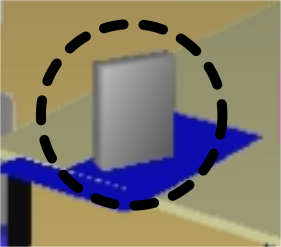
\includegraphics{wait_for_pick}};
            \end{tikzpicture}
        };

        \node[anchor=north] at (ph2 -| ahuman) (wait2) {%
            \begin{tikzpicture}
                \node (title) {\it wait for put\\ {\tt TAPE} to {\tt BIN}};
                \node[below=0.1 of title] {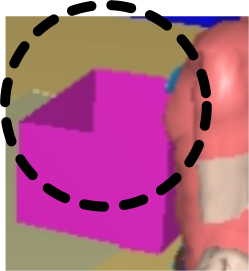
\includegraphics{wait_for_throw}};
            \end{tikzpicture}
        };


        %%%%%%%%%%%%%%%%%%%%%%%%%%%%%%%%%%%%%%%%%%%%%%%%%%%%%%%%%%%%%%%%%%%%%%%%%%%%%%%%%%%%%%%%%%%%
        %%% FLOW
        %%%%%%%%%%%%%%%%%%%%%%%%%%%%%%%%%%%%%%%%%%%%%%%%%%%%%%%%%%%%%%%%%%%%%%%%%%%%%%%%%%%%%%%%%%%%
        \draw[dotted, ->, in=45, out=180] (incoming.west) to (kb1);
        \draw[dotted, ->, bend right] (kb1) to (pr1);
        \draw[dotted, ->, bend left] (pr1) to (ep1);
        \draw[dotted, ->, in=45, out=180] (ae1.west) to (kb2);
        \draw[dotted, ->, bend right] (kb2) to (pr2);
        \draw[dotted, ->, bend left] (pr2) to (ep2);
        \draw[dotted, ->, in=45, out=180] (ae2.west) to (kb3);
        \draw[dotted, ->, bend right] (kb3) to (ph1);
        \draw[dotted, ->, bend left] (ph1) to (wait1);
        \draw[dotted, ->, in=-20, out=180] (wait1.west) to (kb4.east);
        \draw[dotted, ->, bend right] (kb4) to (ph2);
        \draw[dotted, ->, bend left] (ph2) to (wait2);
        \draw[dotted, ->, in=20, out=180] (wait2.west) to (kb5);
        \draw[dotted, ->, bend left] (kb5.east) to (done.north);


 \end{tikzpicture}
 }
 \caption {Chronology of the \emph{Cleaning the table} scenario. The light
     arrows indicate the general flow. This figure
     represents a simplified version: only one object, {\tt TAPE}, must
     be removed from the table and placed in the bin {\tt BIN}.  }
  \label{fig|cleantable-timeline}
\end{figure*}


%The plan produced in that case by HATP is straightforward and shown in the
%third row. It consists of four successive actions involving the robot and the
%human. Robot grasps the tape and then places it on the table at a position
%where it is visible and reachable for the human. The human is then asked to pick
%the tape and throw it in the trashbin.

%%%%%%%%%%%%%%%%%%%%%%%%%%%%%%%%%%%%%%%%%%%%%%%%%%%%%%%%%%%%%%%%%%%%%%%%%%%%%%%%
%%%%%%%%%%%%%%%%%%%%%%%%%%%%%%%%%%%%%%%%%%%%%%%%%%%%%%%%%%%%%%%%%%%%%%%%%%%%%%%%
%%%%%%%%%%%%%%%%%%%%%%%%%%%%%%%%%%%%%%%%%%%%%%%%%%%%%%%%%%%%%%%%%%%%%%%%%%%%%%%%

\section{Discussion: When Artificial Intelligence Enables Human-Robot
Interaction}
\label{sect|conclusion}

This last section tries to clarify the ``take home'' message: what are the challenges
that human-robot interaction brings to artificial intelligence, and what is the
current state-of-the-art in this field?

We first restate the challenge of \emph{embodied cognition} and list what we
seen as the main decisional issues that need to be tackled to push forward
human-robot interaction. We then reflect on the importance of knowledge handling
in modern robotics and put our choice of the RDF formalism into perspective.
Finally, we briefly re-discuss two facets of HRI: the importance of
\emph{modelling the humans}, and the difficulty of \emph{acting in presence of
humans}.

\subsection{Embodied Cognition}

Robotics is traditionally regarded as the prototypical instance of \emph{embodied}
artificial intelligence, and this dimension is especially prevalent in
human-robot interaction, where agents have to share a joint physical
environment.

It results in a tight coupling between the symbolic and the geometric realms:
while AI at its origins was mostly a matter of symbolic models, it has been
since recognised that not only the mind is not a purely abstract system,
disconnected from the physical world, but even more, cognition fundamentally
relies on its relation to the physical world (so-called \emph{embodied
cognition}). Varela~\cite{Varela1992} is one of the main discoverer of these
mechanisms, and coined the concept of \emph{enactivism} as the theoretical
framework that study the links between cognition, embodiment and actions.

The challenge of symbol grounding is tightly linked to this issue. It
corresponds to the identification or creation, and then, maintenance of a link
between the symbol (the syntactic form of knowledge the computer will
manipulate) and its semantics, \ie its meaning, anchored in the world (the
relations between the symbol, the referent of the symbol, and mediating minds
is classically referred as the \emph{semantic triangle}, and has been
extensively studied in linguistics). The issue of grounding is well known in
cognitive science and is summarised by Harnard~\cite{Harnad1990} by this
question: ``how the semantic interpretation of a formal symbol system can be
made intrinsic to the system?''. This issue has a major practical importance in
robotic: for a robot to be both endowed with a symbolic representational and
reasoning system, and able to \emph{act} in the physical world, it must ground
its knowledge.

Grounding is implemented at different levels in our architecture. The main source
of grounded symbolic knowledge is the situation assessment module, {\sc Spark}.
Not only it builds symbolic facts from spatial reasoning, but it also relies on
temporal reasoning to track the world state and build explanations to interpret
unexpected perceptions (we mentioned above the example of a disappearing
object).

Because {\sc Spark} is also able to track humans, which enables in turn
perspective-aware spatial reasoning, it produces grounded symbolic knowledge
for interacting agents as well. This is a typical \emph{embodied} cognitive
skill.

Grounding also occurs during verbal and non-verbal communication. The {\sc
Dialogs} module grounds new concepts introduced by the speaker by asking questions
until it can attach the new concept to concepts already present in the
knowledge pool (typically, if I ask the robot ``bring me a platypus'', the
robot asks ``what is a platypus''. I may answer ``a mammal'' and the robot will
ask ``what is a mammal?'' and so on until it anchors the new concepts to ones
it already knows). Non verbal interaction (like gestures) is also partially
grounded. When the user points at something, it can say ``give me this'' and
the robot grounds \emph{this} to the pointed artifact.

Because only objects marked with tags are currently recognised (in our typical
lab experiments, it may be a dozen of them), the robot grounding mechanisms work
in a small-sized closed world. This assumption obviously greatly facilitates
the task. It remains to be seen if systematic marking of manipulated objects
(for instance with RFID tags) is a realistic path. It may be the case if the
robot is expected to be used in a well-defined, slowly changing environment.
Real-time recognition of large libraries of objects is another path which may
be viable soon~\cite{Dean2013Fast}.

\subsection{The Key Decisional Issues}

How can we restate the main challenges, in particular in term of decision
making, that human-robot interaction brings to artificial intelligence?

\fxfatal{TDB}



\subsection{Knowledge and Robotics}
\label{krs-discussion}


\subsubsection{Knowledge and Architecture}

As a whole, the components that we have introduced so far build a
knowledge-oriented architecture: Knowledge is explicitly stored in one central
and consistent repository of facts, accessible for all modules. It relies on a
\emph{strict formalism} (OWL statements), with a \emph{well defined vocabulary}
(stated in the common-sense ontology). These first two points lead to a
\emph{loosely-coupled architecture} where modules can be removed or replaced
easily by other ones as long as they share the same semantics (modules are
defined by the knowledge they produce).

Also, we adopt a symbolic, reactive, event-driven approach to robot control. By
managing events at the same level as the reasoner, we take full advantage of the
inference abilities of {\sc Oro} to trigger events whose \texttt{true}
conditions can be inferred.

And finally, this architecture allows for the combination of very different
knowledge modalities in a single homogeneous environment, bringing mutual
benefits to components. For instance, the dialogue processing module can
perfectly run without any geometric perception, but its disambiguation routines
can transparently benefit from it when available (since richer symbolic
descriptions of objects are then available).

Those items are not new \emph{per se}. It is however interesting to underline
the shift of focus this implies during the design and integration phases of
robots: components of our deliberative layer are defined and glued together by
the knowledge they produce and consume. Human-robot interaction, because it
supposes operations at \emph{human-level} and in environments with complex
semantics, acts here as a motivational force.

\subsubsection{RDF as a Formalism for Semantics}

Knowledge flows in our architecture through a \emph{semantic blackboard}, the
{\sc Oro} server. We rely on Description Logics (OWL) to represent and
manipulate facts.

Relying on RDF triples and Description Logics has advantages such as good
understanding of its trades-off, thanks to being widespread in the semantic Web
community, the availability of mature libraries to manipulate the ontology,
interoperability with several major on-line knowledge bases ({\sc
OpenCyc}, {\sc WordNet}, {\sc DBPedia} or {\sc RoboEarth}~\cite{Waibel2011} are
some examples), open-world reasoning, and the formal guarantee of decidability
(it is always possible to classify a Description Logics ontology).

It also has notable limitations, both fundamental (the suitability of
Description Logics when reasoning on --typically non-monotonic-- commonsense
knowledge is questionable) and practical: RDF triples imply only binary
predicates, which constrains the expressiveness of the system or leads to
cumbersome reifications. Alternatives exist (like {\sc
KnowRob}~\cite{Tenorth2009a}) that mix RDF with more expressive logic languages
like {\sc Prolog} with other limitations, like closed-world reasoning. The
classification performance is another issue: from our experience, with an
ontology sized for a standard experiment (about 100 classes and 200 instances),
classification typically takes about 100ms, which becomes problematic during
interactions.  Besides, the performances are difficult to predict, since a
seemingly inoffensive new statement may indirectly change abruptly the logical
complexity of the whole knowledge model and lead to notable degradation of
classification time.

This knowledge model also largely excludes representation of continuous
phenomena (like time) or uncertain phenomena. When required (for instance for
action recognition), these are managed by dedicated components (like {\sc
Spark}), and are not exposed at the semantic level.

Alternatives like \emph{Answer Set Programming} have also been
successfully investigated in robotics~\cite{Chen2010,Erdem2012}, in particular
to deal with non-monotonic reasoning. However we did not actually hit any brick wall
while working with OWL ontologies. We may reconsider this choice at a later
stage, but until now it has proven an effective framework to quickly explore
implementations of new cognitive abilities (for instance, it has been
conceptually and technically easy to add support for independent knowledge
models, one per agent the robot interacts with --see section~\ref{sect|tom}).

Besides, because ontologies and RDF statements are relatively simple concepts
to grasp, it also effectively helped to grow awareness amongst colleagues on
the significance of the ``semantic level'' when developing new components for
the robot.


\subsection{Bringing the Humans into the Equation}

\subsubsection{Modelling the Humans}

Perspective taking is this human ability which allows one to put him/herself in
another person's point of view. Studied in psychology
literature~\cite{Flavell1992,Tversky1999}, this ability is crucial when
interacting with people by allowing one to reason on others' understanding of
the world in terms of visual perception, spatial descriptions, affordances and
beliefs, etc.  In the last years these notions have been gradually employed in
HRI.~\cite{Breazeal2006} presents a learning algorithm that takes into account
information about a teacher's visual perspective in order to learn a task.
~\cite{Johnson2005} apply visual perspective taking for action recognition
between two robots.~\cite{Trafton2005} use both visual and spatial perspective
taking to find out the referent indicated by a human partner.

In our implementation, perspective taking is tightly connected to the symbolic
knowledge models, and since our knowledge base allows for storage of one
knowledge model per agent, we have been able to endow the robot with a simple
theory of mind (as explained in section~\ref{sect|tom}): we explicitly model
what the robot knows about its partners in a symbolic way. This knowledge is
then re-used in different places, to correctly interpret what the human says,
or to plan tasks that are actually doable for the human.

The cognitive model that the robot builds for the agent it interacts with is
still simple and mostly focused on geometric features (\emph{Who sees what? What are
our relative positions?} etc.). Extending this knowledge with more subtle
perceptions (emotional state for instance) remains to be done.

We should also mention that modelling of human behaviours also appear in our
architecture at the level of task and motion planning with a set of
\emph{social rules}, including proxemics, action legibility or time
optimization.

\subsubsection{Acting in Presence of Humans}

HRI offers new challenges to planning
by adding a complementary constraint: the synthesis of plans that are not only
feasible but legible (in terms of their intention) and compliant with human
preferences. This constraint is often ill-defined, dynamic, context-dependent.

Indeed, we posit that human-robot collaborative task achievement calls for more
subtlety for a robot than autonomous independent task achievement. HATP, by
co-planning for the robot and the human, and modelling social rules as planning
parameters, is a first step in this direction.

\paragraph{Joint actions with humans}\label{sec:soa}
The human presence brings new requirements for robot's abilities both
at the functional and at the deliberative levels~\cite{Klein2004}. The
topics involve motion~\cite{Kulic2007,Berg2004,Madhava2006},
navigation~\cite{Althaus2004,Sisbot2007}, manipulation~\cite{Kemp2007}
in presence of humans as well as perception of human
activities~\cite{Breazeal2001,Burger2008}. Also, when
interacting with humans, robots need to incorporate communication and
collaboration abilities. Several theories dealing with
collaboration~\cite{Cohen1991,Grosz1996,Clark1996} emphasise that
collaborative tasks have specific requirements compared to individual
ones, \eg, since the robot and the person share a common goal, they
have to agree on the manner to realise it, they must show their
commitment to the goal during execution, etc. Several robotic systems
have already been built based on these
theories~\cite{Rich1997,Sidner2005,Breazeal2003} and they
all have shown benefits of this approach. They have also shown how
difficult it is to manage turn-taking between communication partners
and to interleave task realization and communication in a generic
way. Finally, today only few
systems~\cite{Fong2006,Breazeal2003,Sisbot2008} take humans into
account at all levels.


\paragraph{Limits of Disambiguation at Semantic Level}

Interaction with humans implies the ability to deal with semantics: semantics of
verbal interaction, semantics of gestures, etc.  As a consequence, it also
implies to deal with semantic disambiguation.

One prototypical example of semantic disambiguation has been given in
\cite{Ros2010b} with the child game \emph{spygame}: two players are facing
each other with a set of random objects in-between, one player mentally choose
one object, and the other player has to guess the object by asking closed
questions like \emph{Is your object small or large?} Based on the knowledge it
has acquired, the robot is able to minimise the number of questions required to
find the object.

When playing this kind of game, however, the issue arises that the robot has no
way to select which knowledge about the object is relevant in the interaction
context. For instance, the knowledge base may store facts like \stmt{obj1 type
ActiveConcept} (which internally means that this concept was mentioned in a
discussion in the last few seconds): this information is not a relevant
property of \concept{obj1} when trying to disambiguate concepts with humans.
This distinction between \emph{internal knowledge} (meaningful to
the system only) and \emph{common knowledge} (whose meaning is understood by
all the interactors) has not been properly dealt with in our architecture.

Besides, even knowledge that belongs to the \emph{common knowledge} may not be
appropriate in a given interaction context. For instance, the system may
compute that at a given instant the human is looking at the object: \stmt{human
looksAt obj1}. This property makes sense to both parties, but in the context of
the \emph{spygame}, we would like to mainly use immanent properties, not
volatile like a gaze. More research is required to identify relevant
interaction contexts and knowledge classes attached to them.

\subsection{The Next Steps}

%We have presented in this article a decisional framework for human-robot
%interactive task achievement that is aimed to allow the robot not only to
%accomplish its tasks but also to produce behaviours that support its engagement
%vis-a-vis its human partner and to interpret human behaviours and intentions.
%Together and in coherence with this framework, we have developed and
%experimented various task planners and interaction schemes that allow the robot
%to select and perform its tasks while taking into account explicitly the human
%abilities as well as the constraints imposed by the presence of humans, their
%needs and preferences. 

The design choices and the results presented here are still preliminary.
While the general scheme we propose might be difficult to implement in
a general sense, we believe that it is a reasonable challenge to
implement it in the case of a personal robot assistant essentially
devoted to fetch-and-carry, as well as for interactive manipulation
tasks and associated activities.

One direction that we would like to further investigate is how to account for
situations where divergent beliefs appear between the human and the robot.
Preliminary results have been published in~\cite{warnier2012when}.

There is also extensive work to be done in order to refine the notion of ``good
shared plan'' and ``good/acceptable robot behaviour'' in this context. There are
obviously large avenues for learning and adaptation in this context.

Another broader direction to head deals with \emph{contexts representation}.
Contexts are currently often limited to the current spatial and temporal
situation. Some projects model offer the possibility to jump in the past or to
switch to another agent's perspective, but in current approaches, selecting a
context always basically consists in retrieving a set of beliefs corresponding
to a situation, and temporarily replacing the current beliefs by those other
ones. This misses the fact that at a given moment, not one but many contexts
co-exist at different scales. We do not want to retrieve one monolithic set of
beliefs, but instead carefully craft a context from several \emph{atomic}
contexts. Techniques for representation of overlapping pools of knowledge
largely remain to be developed, as well as efficient algorithms to retrieve (or
discard) such context-related pools of knowledge. This is a challenge not only
for robotics, but more generally for artificial intelligence.

The ability to explicitly manage contexts and context switches would endow the
robot with a cognitive capability similar to what is known as
\emph{context-dependent memory} in cognitive psychology. This is also related
to Tulving's \emph{autonoetic consciousness}~\cite{Tulving1985a}: the ability
to reflect upon its own past or future experiences.

Much remain to be done to this regard, starting with a formal analysis of what
are the relevant contexts for our robots.

Human-Robot Interaction is and is going to remain a challenging field for
artificial intelligence. We hope that this contribution helps with clarifying
some of these challenges.

\section*{Acknowledgements}

Building such a robotic architecture is the work of many hands, and we would
like to acknowledge here the worthwhile contributions of Samir Alili, Aurélie
Clodic, Raquel Ros Espinoza, Mamoun Gharbi, Julien Guitton, Matthieu Herrb, Jim
Mainprice and Amit Kumar Pandey.

This work has been supported by EU FP7 ``SAPHARI'' under grant agreement no.
ICT-287513.


\bibliographystyle{elsarticle-num}
%\bibliographystyle{abbrv}
\bibliography{laas_hri}



\end{document}
